%------------------------------------------------------------------------------
\chapter{Front-end electronics}
\label{sec:appendixFE_electronics}
%------------------------------------------------------------------------------

%% \section{Energy calibration}\label{sec:appendix_energy_calibration}

%% \begin{figure}[htbp] \centering
%%   \begin{subfigure}[b]{0.45\textwidth}
%%     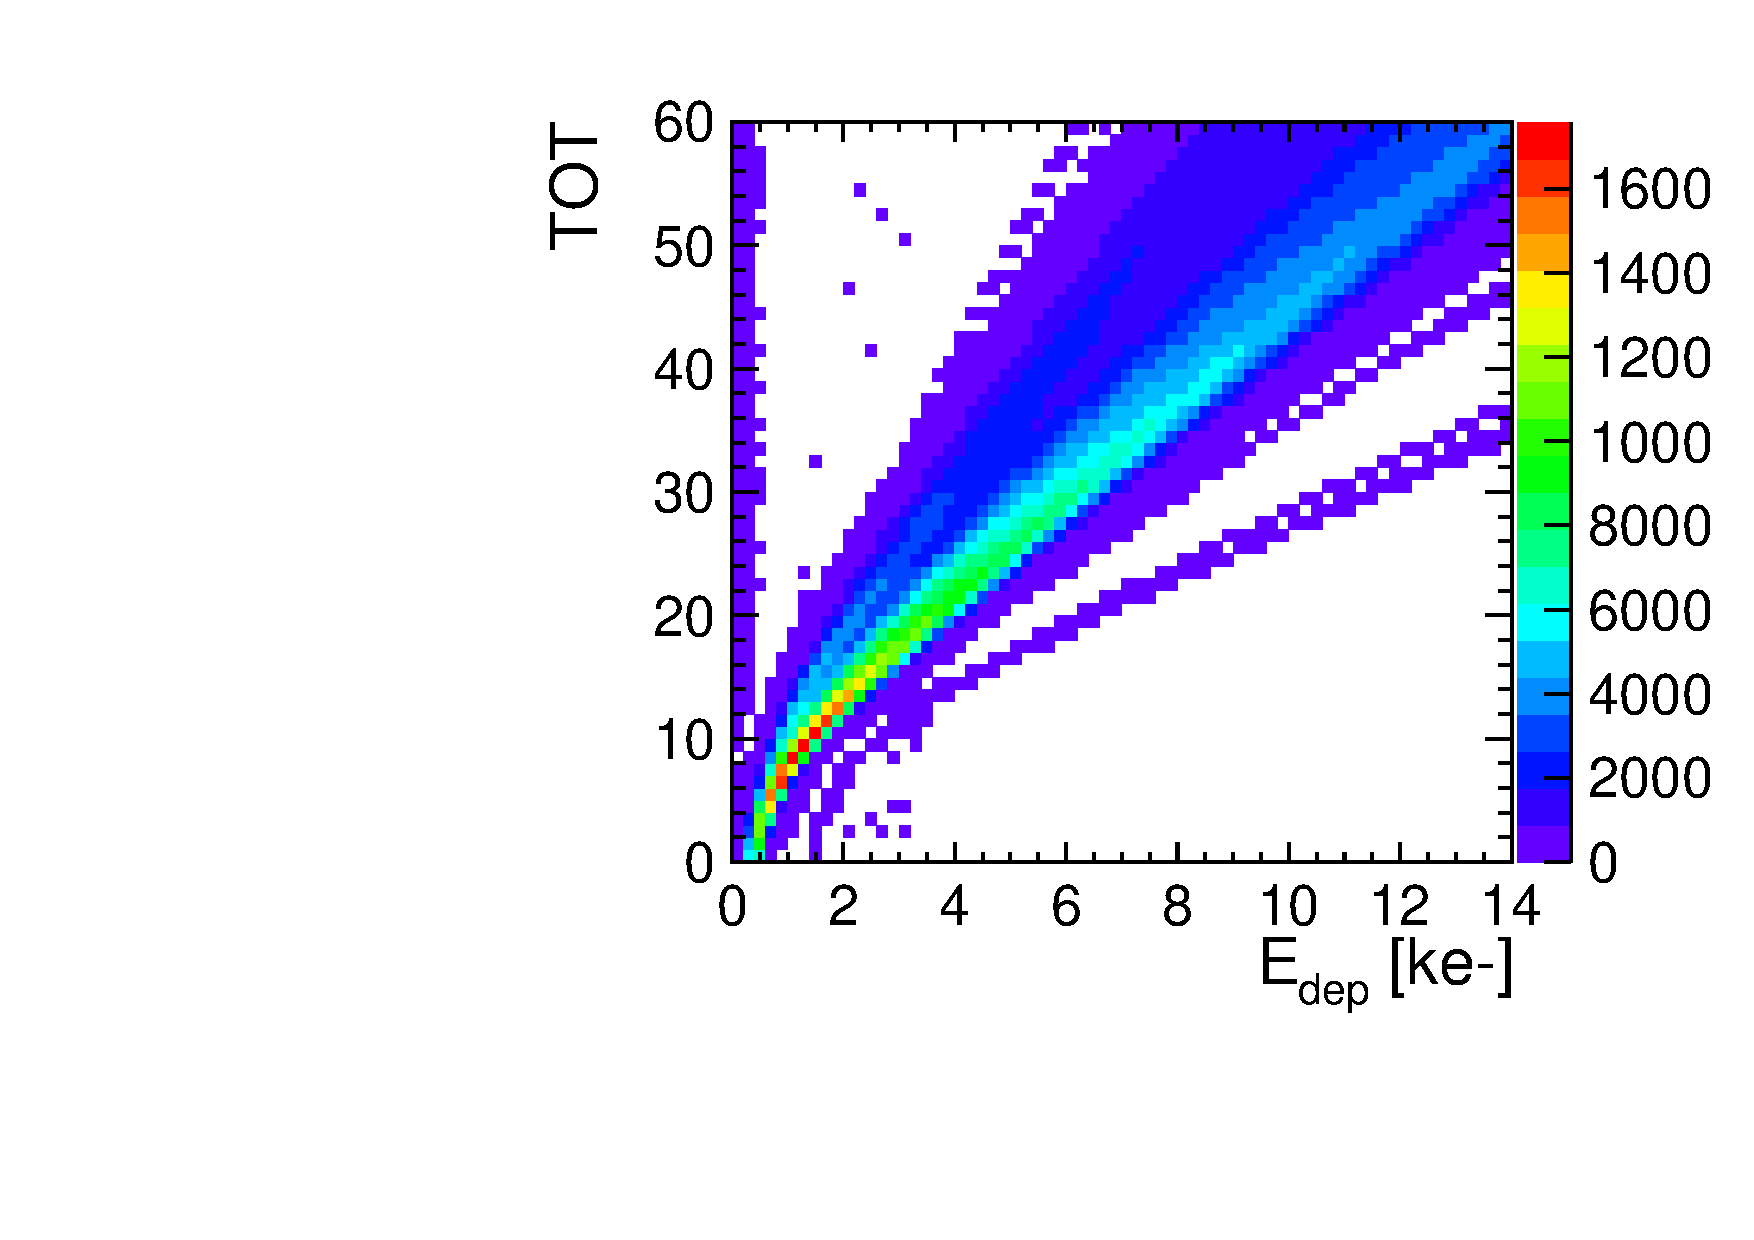
\includegraphics[width=\textwidth]{./figures/Calibration/TOTcalibration_W0005_F01_thresh1153.pdf}
%%     \caption{TOT calibration for W5\_F1, THL=1153.}
%%     \label{fig:TOTcalibW5F1}
%%   \end{subfigure}\hfill
%%   \begin{subfigure}[b]{0.45\textwidth}
%%     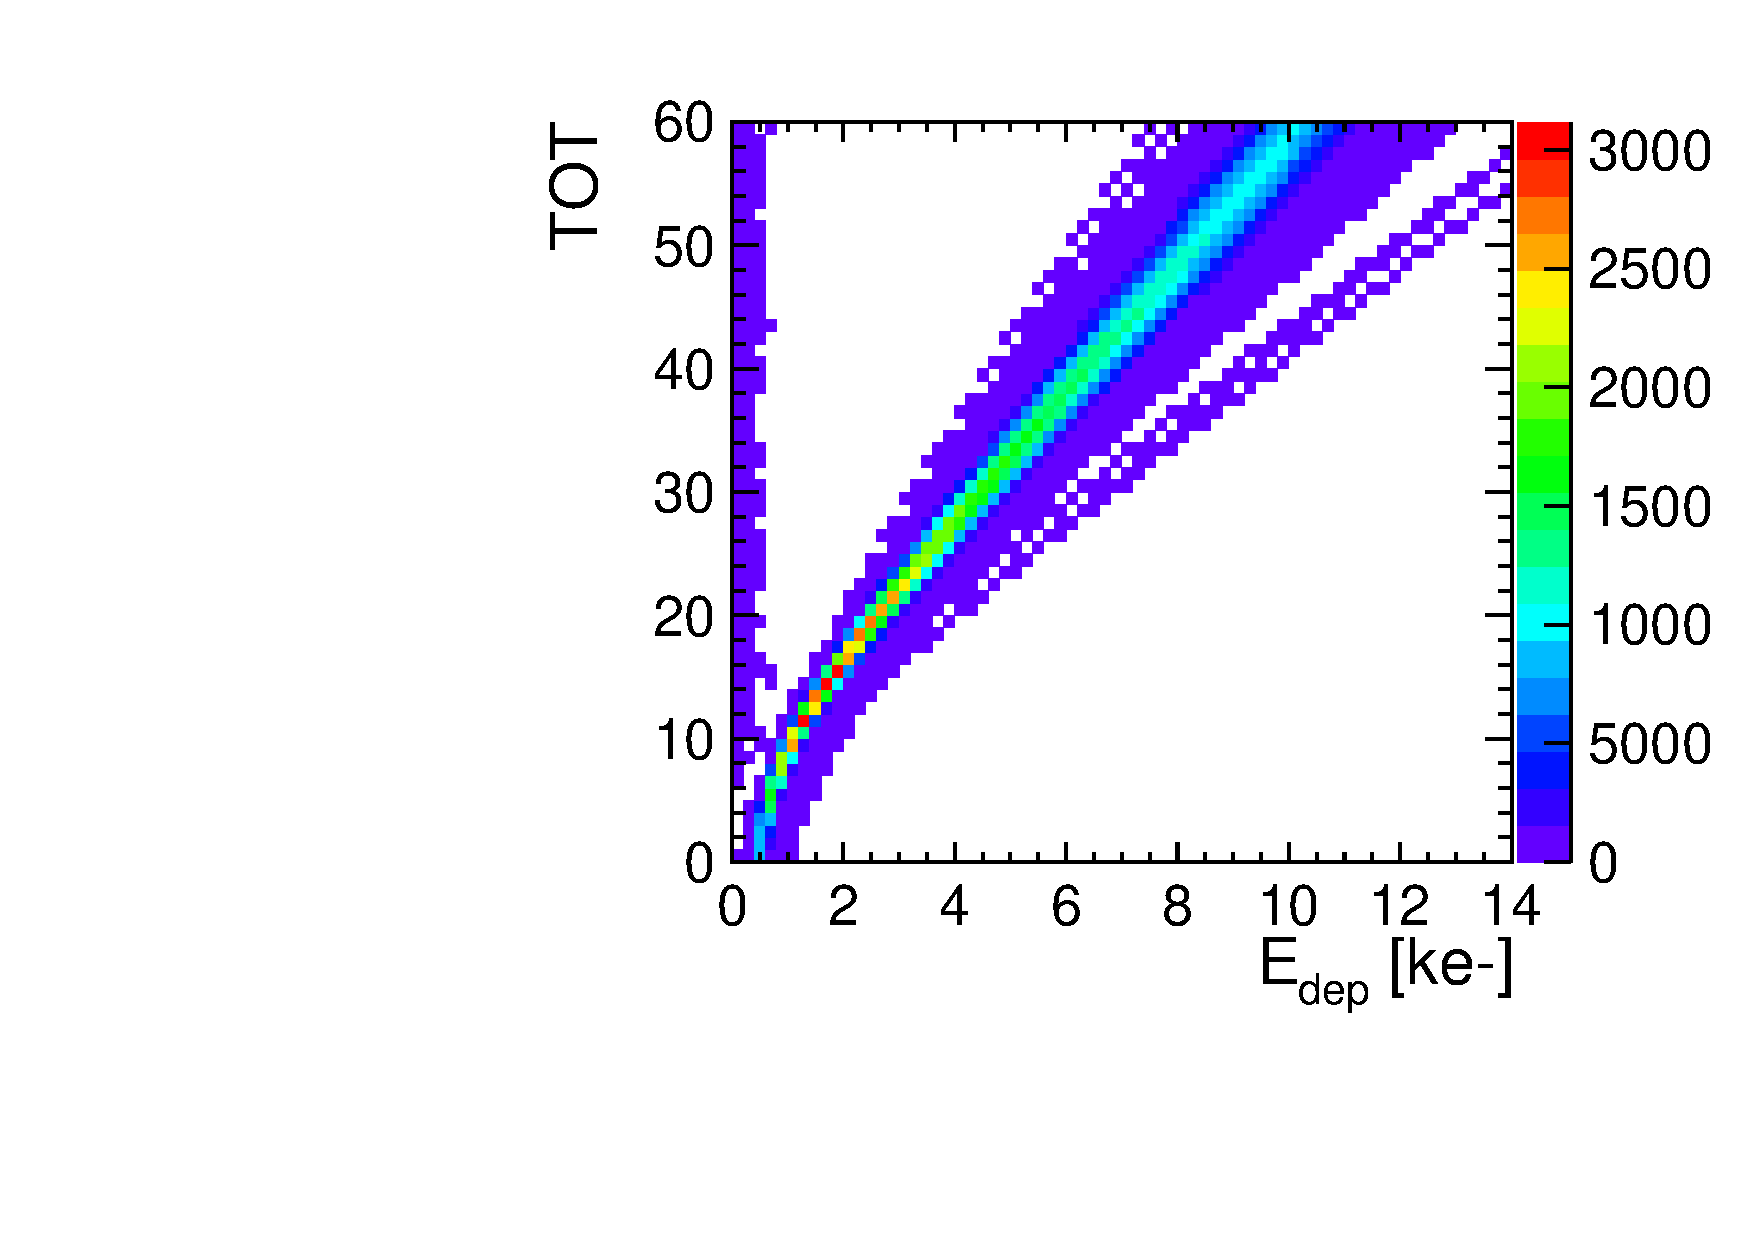
\includegraphics[width=\textwidth]{./figures/Calibration/TOTcalibration_W0019_C07_thresh1148.pdf}
%%     \caption{TOT calibration for W19\_C7, THL=1148.}
%%     \label{fig:TOTcalibW19C7}
%%   \end{subfigure}
%% \end{figure}


%% \begin{figure}[htbp] \centering
%%   \begin{subfigure}[b]{0.45\textwidth}
%%     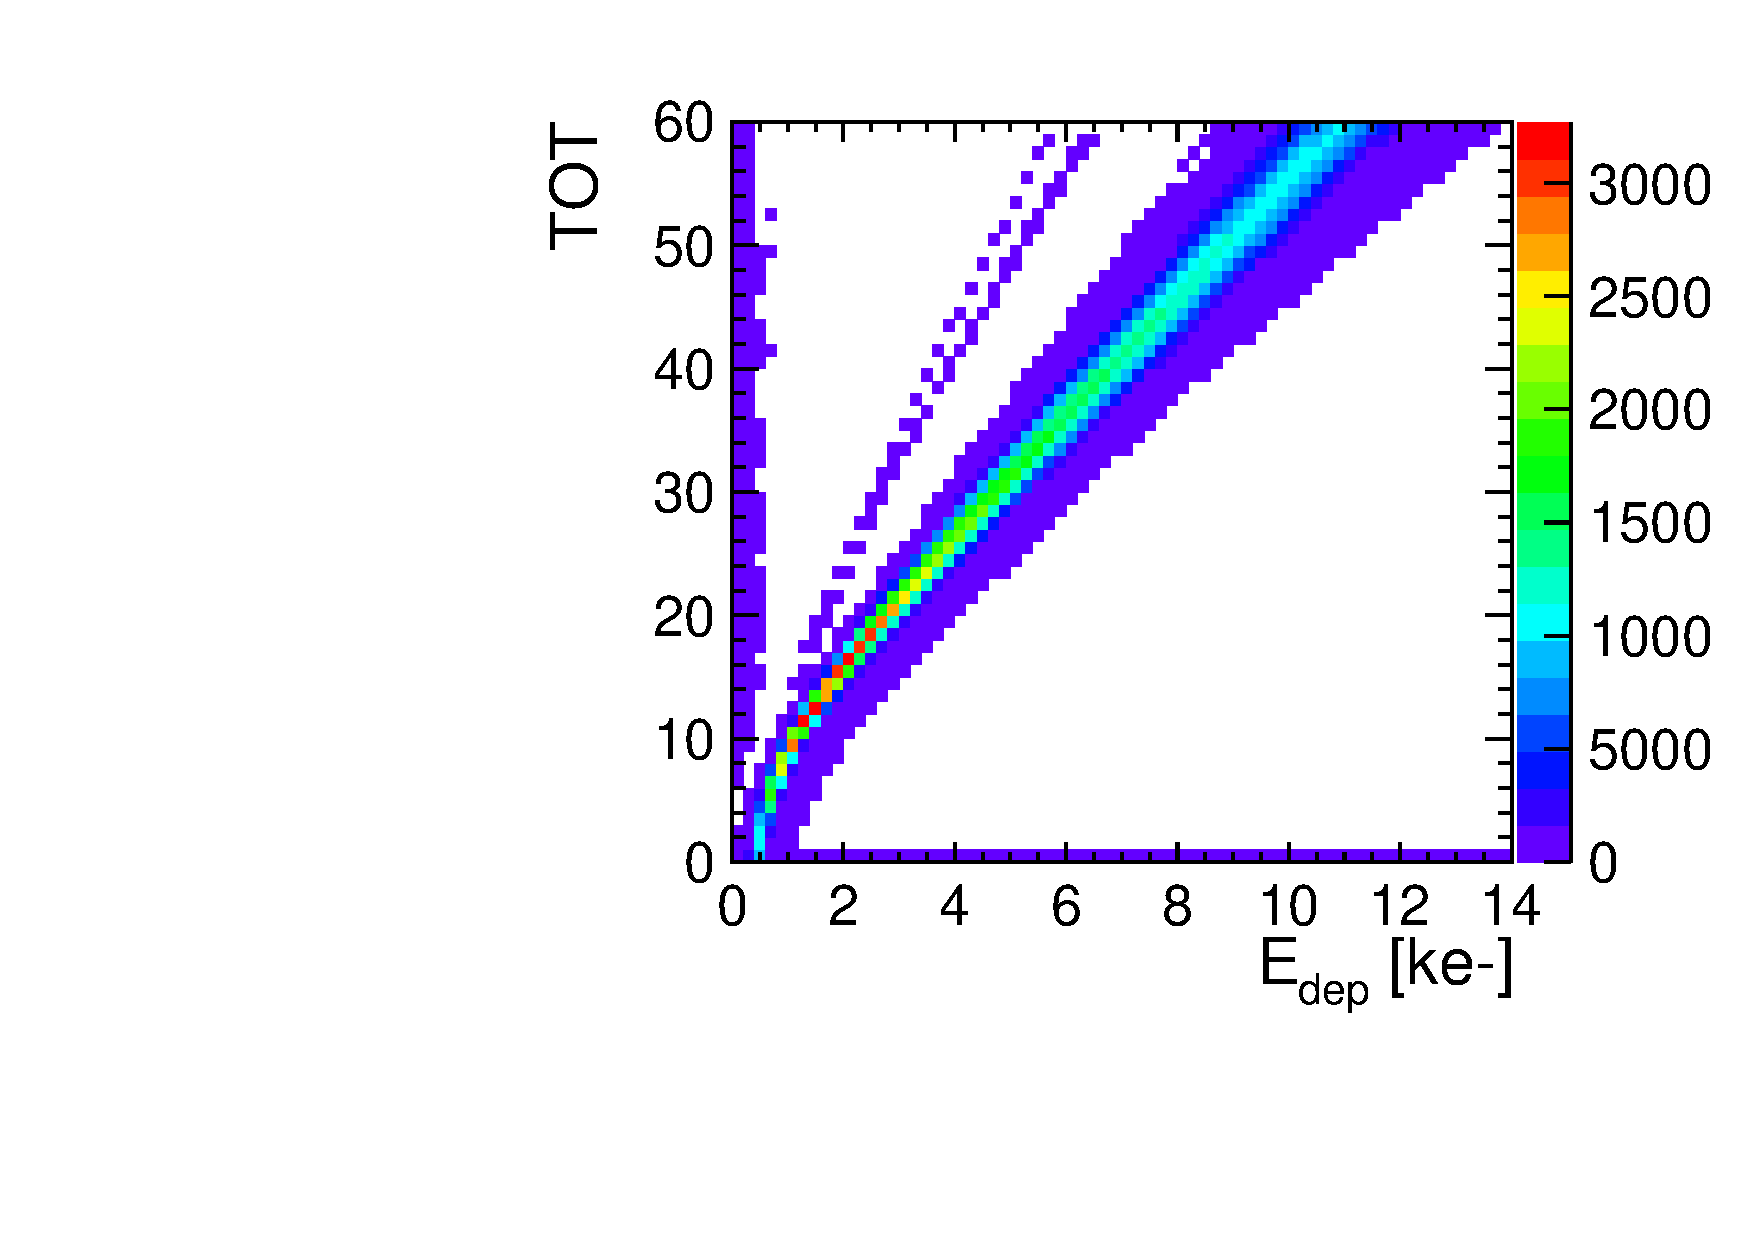
\includegraphics[width=\textwidth]{./figures/Calibration/TOTcalibration_W0019_G07_thresh1190.pdf}
%%     \caption{TOT calibration for W19\_G7, THL=1190.}
%%     \label{fig:TOTcalibW19G7}
%%   \end{subfigure}\hfill
%%   \begin{subfigure}[b]{0.45\textwidth}
%%     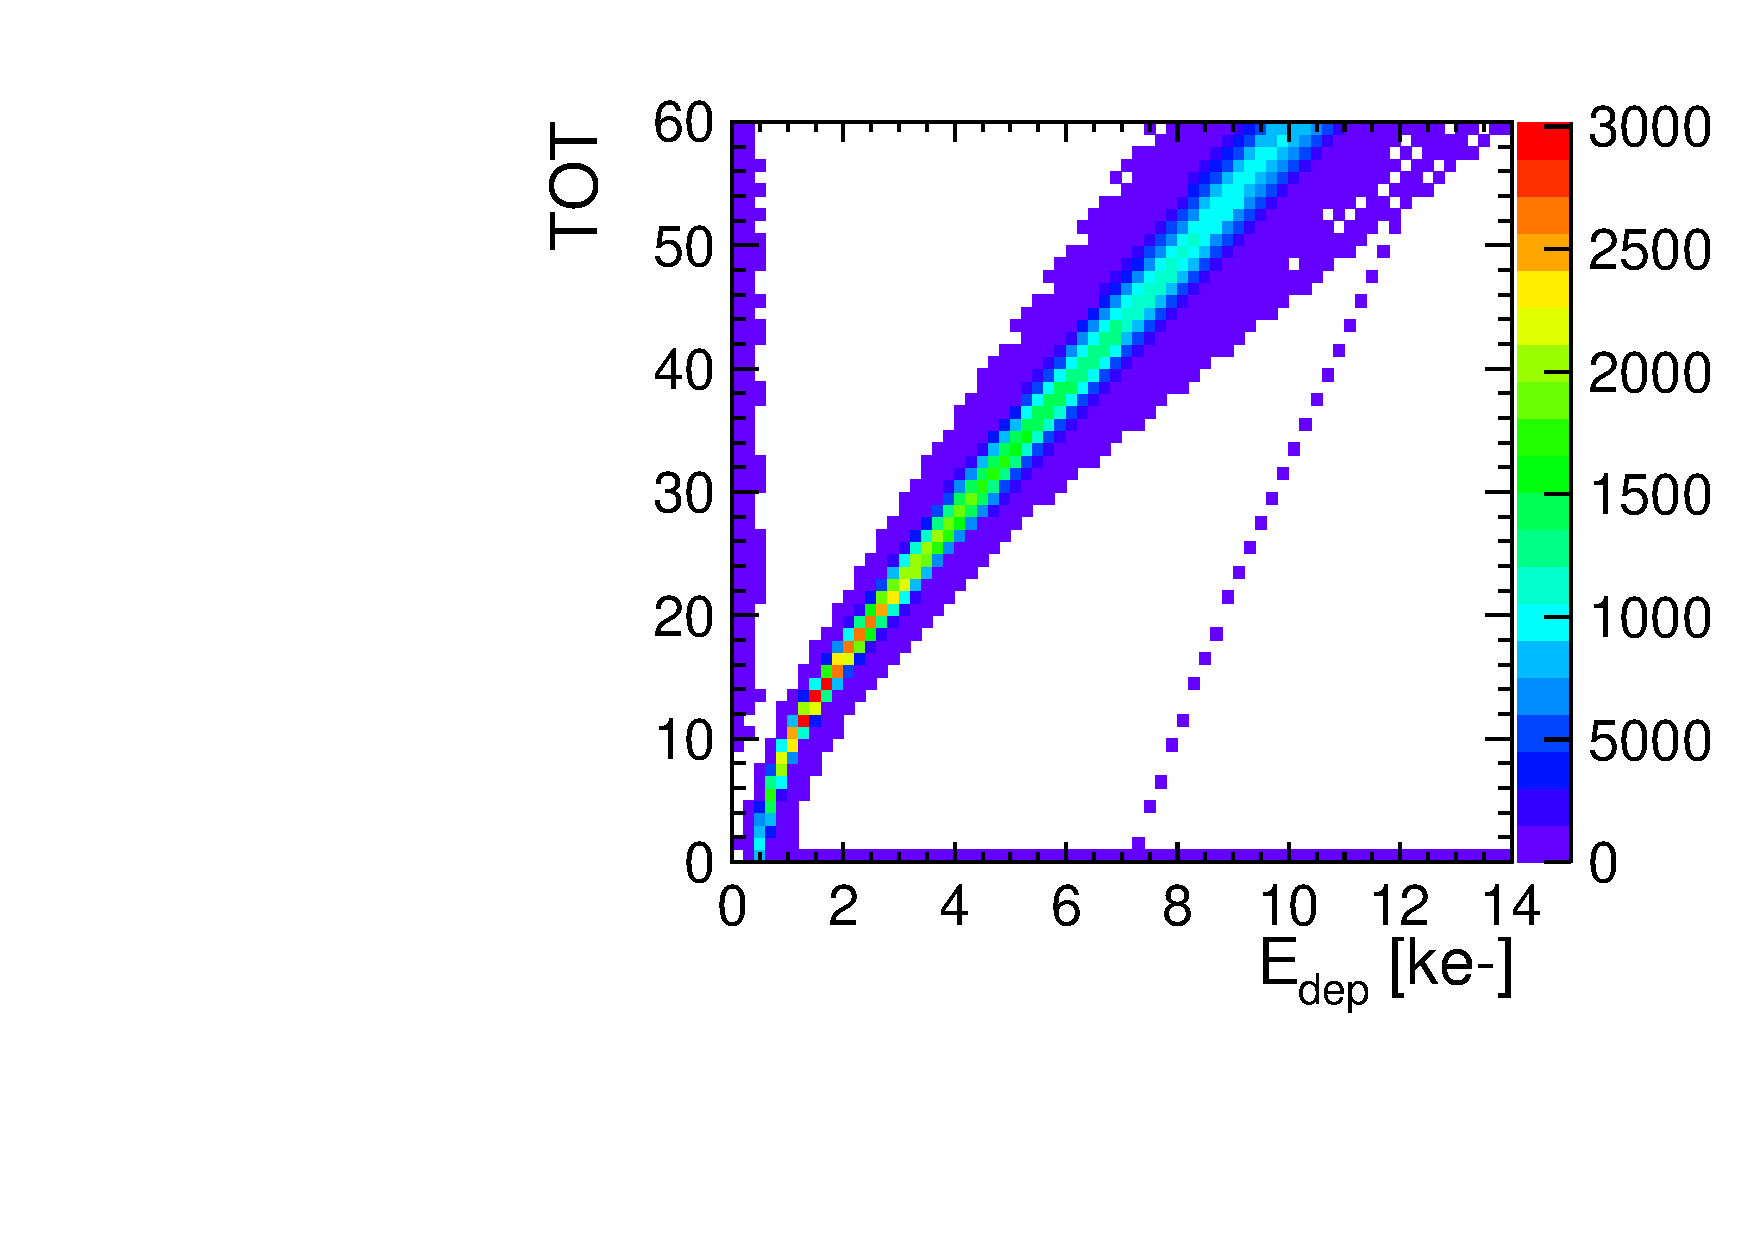
\includegraphics[width=\textwidth]{./figures/Calibration/TOTcalibration_W0019_L08_thresh1133.pdf}
%%     \caption{TOT calibration for W19\_L8, THL=1133.}
%%     \label{fig:TOTcalibW19L8}
%%   \end{subfigure}
%% \end{figure}


\section{Threshold calibration}\label{sec:appendix_threshold_calibration}
\begin{figure}[htbp] \centering
  \begin{subfigure}[b]{0.45\textwidth}
    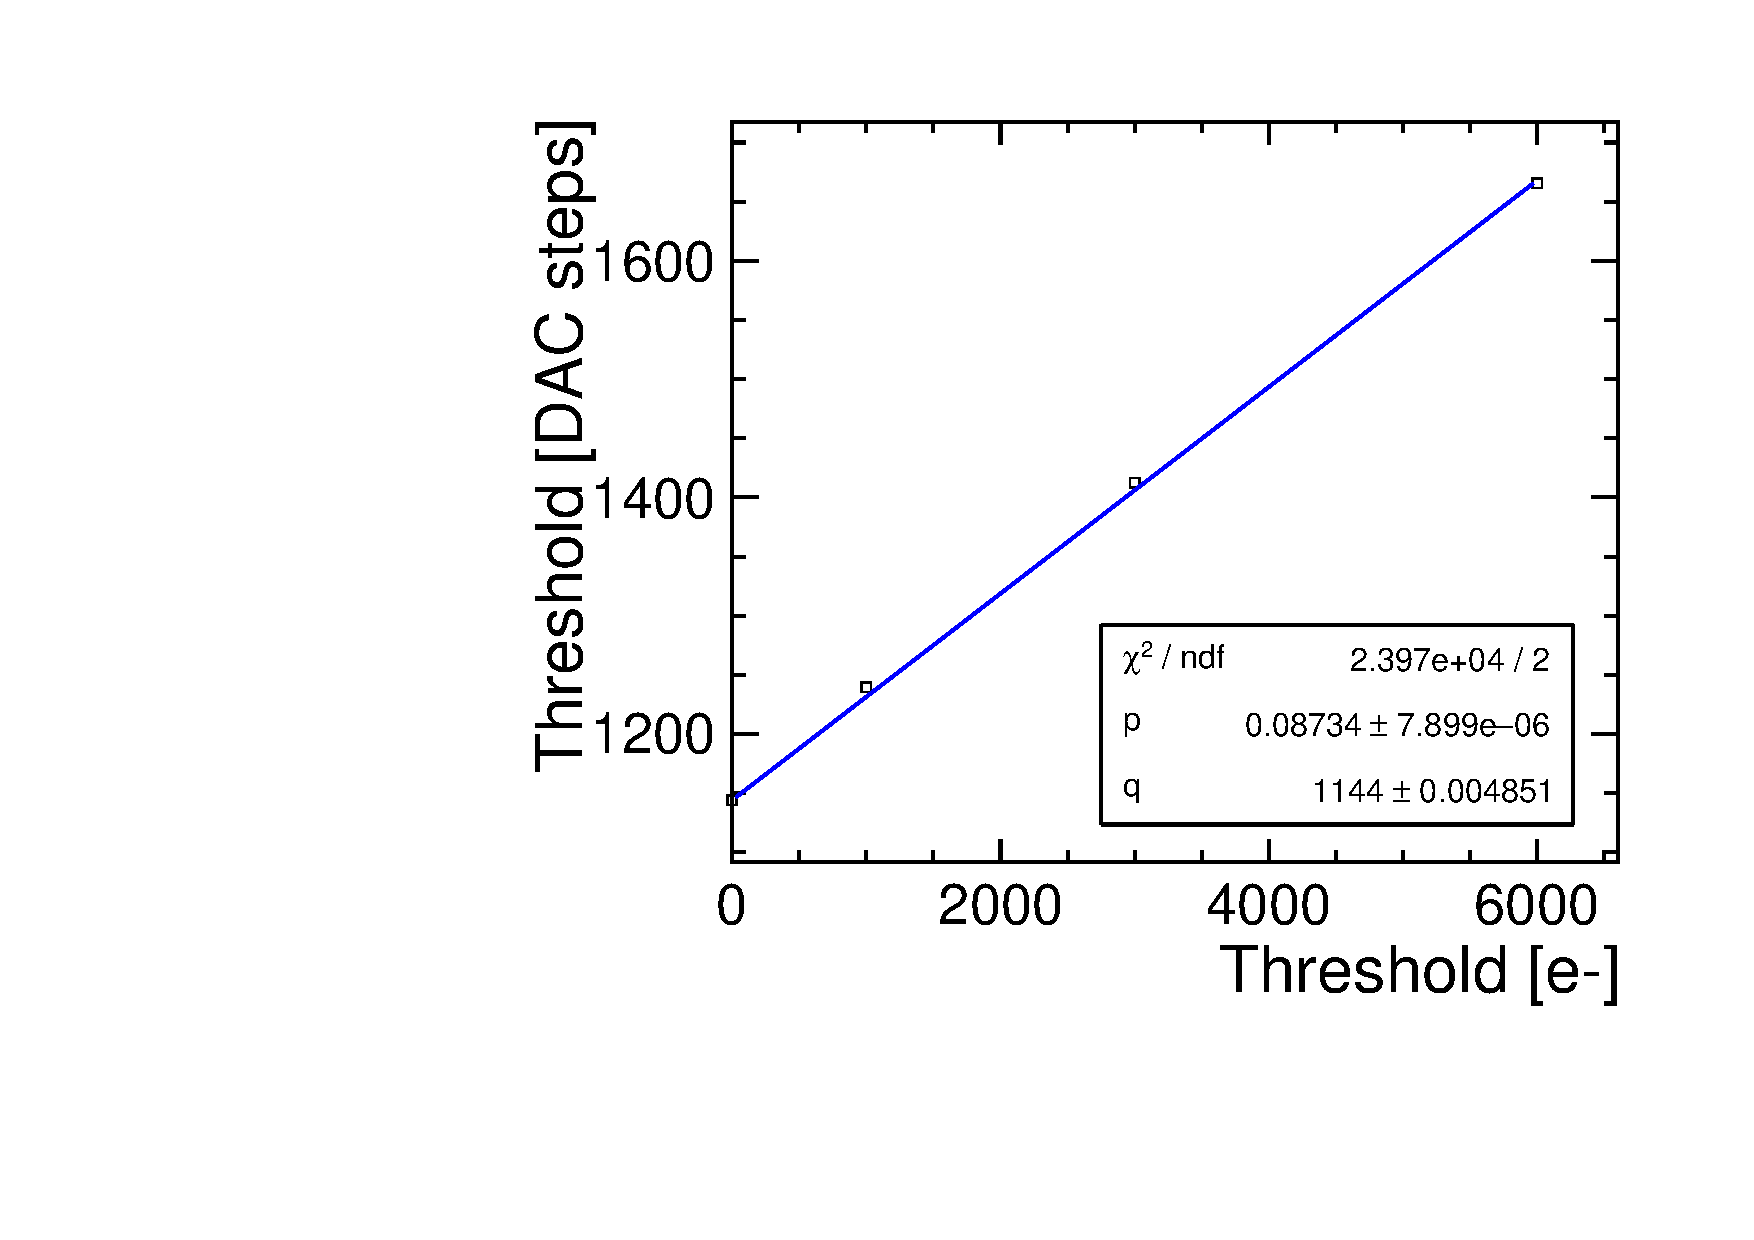
\includegraphics[width=0.9\textwidth]{./figures/Calibration/THLcalibration_W0019_G07.pdf}
    \caption{W19\_G7}
  \end{subfigure} \hfill
  \begin{subfigure}[b]{0.45\textwidth}
    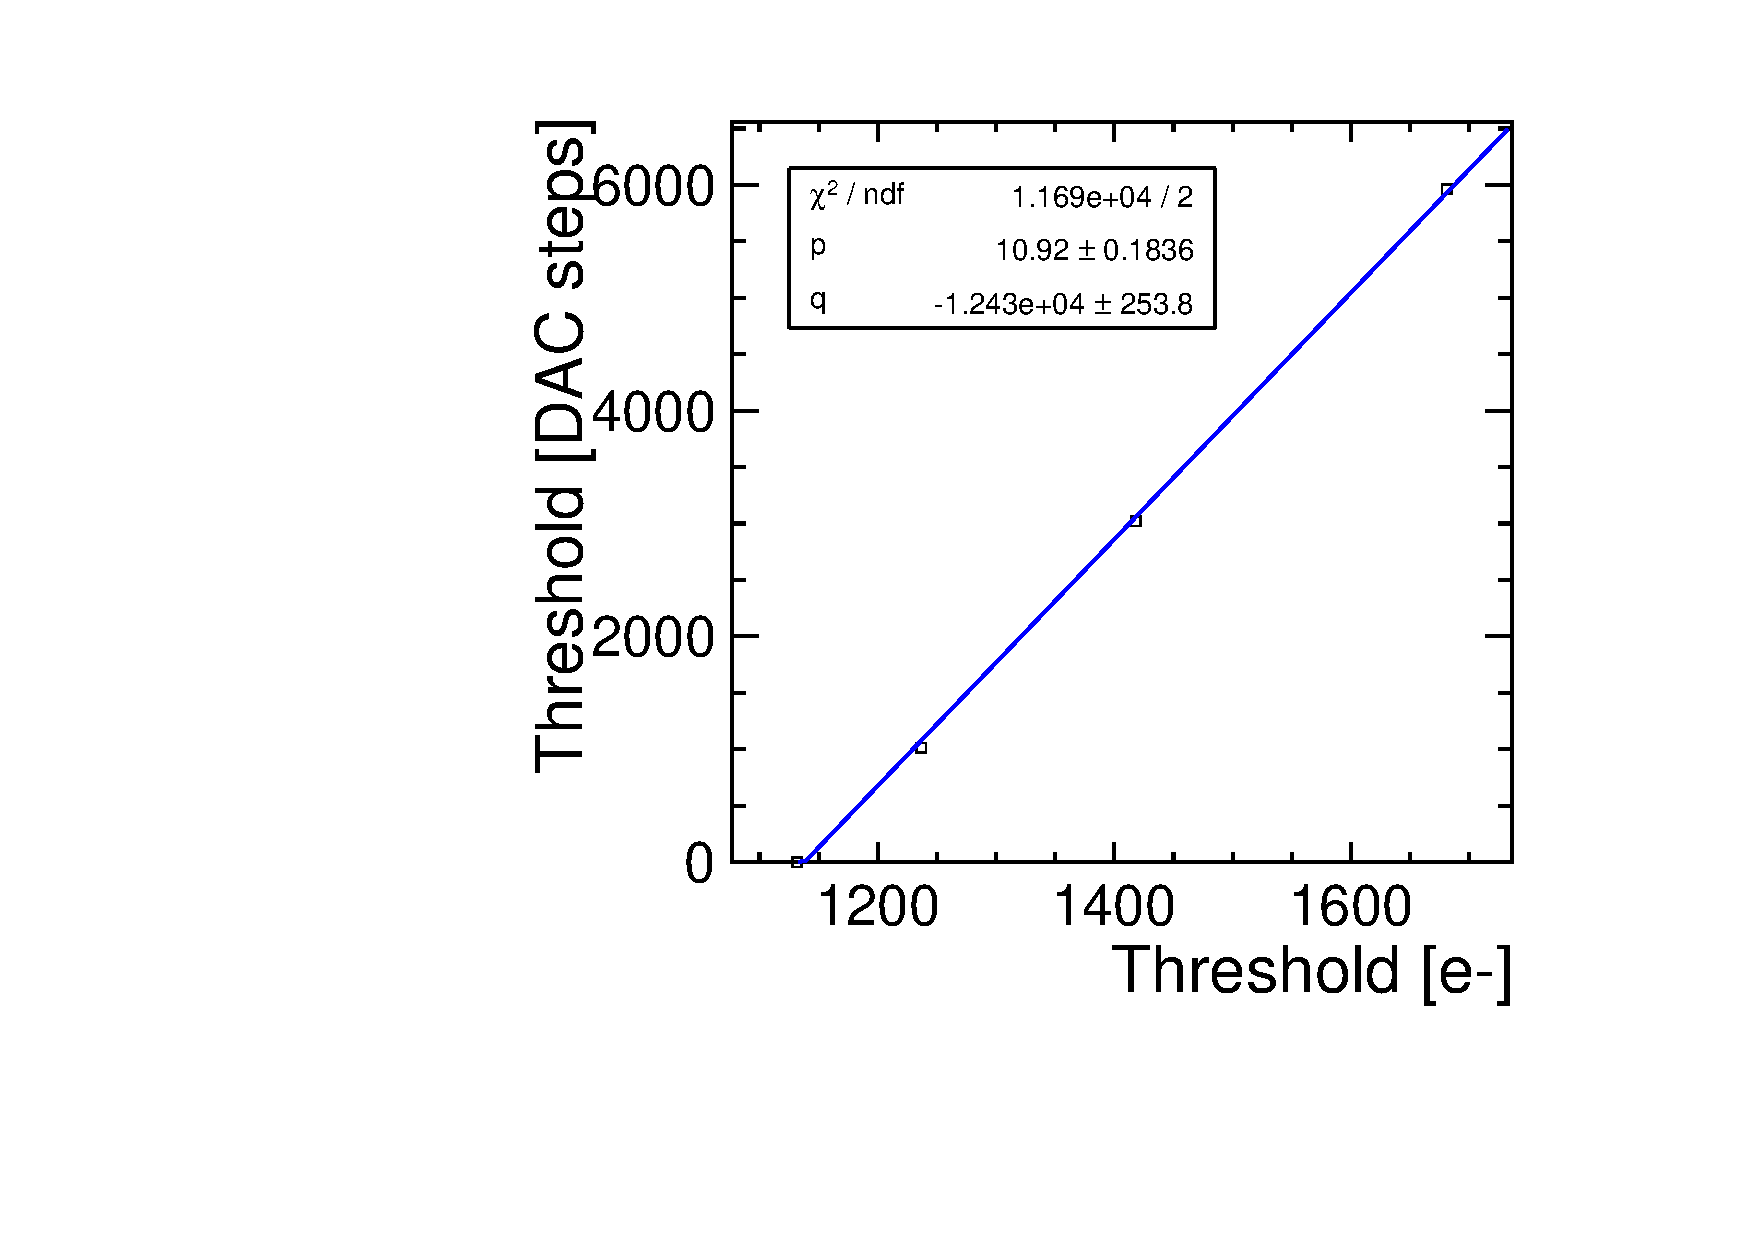
\includegraphics[width=0.9\textwidth]{./figures/Calibration/THLcalibration_W0019_F07.pdf}
    \caption{W19\_F7}
  \end{subfigure}\\
  \begin{subfigure}[b]{0.45\textwidth}
    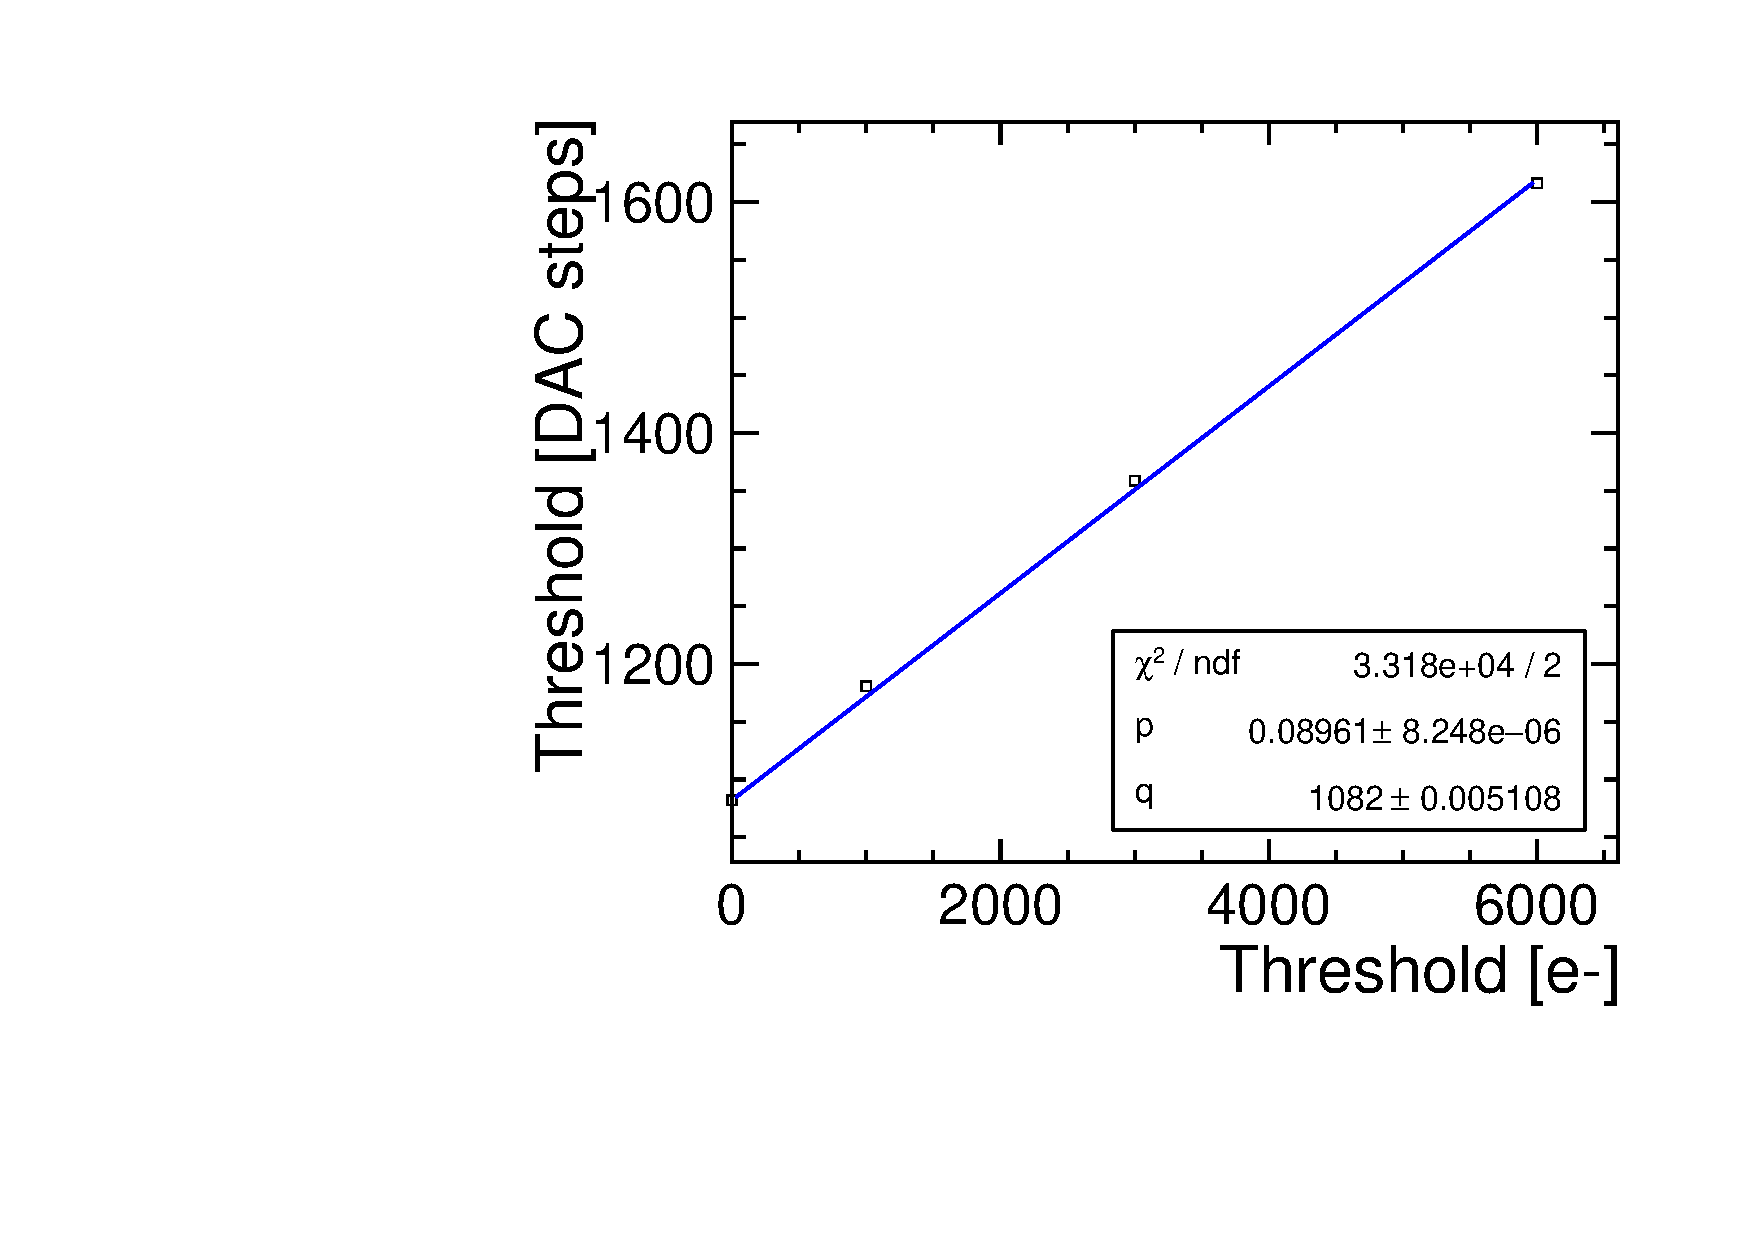
\includegraphics[width=0.9\textwidth]{./figures/Calibration/THLcalibration_W0019_L08.pdf}
    \caption{W19\_L8}
  \end{subfigure} \hfill
  \begin{subfigure}[b]{0.45\textwidth}
    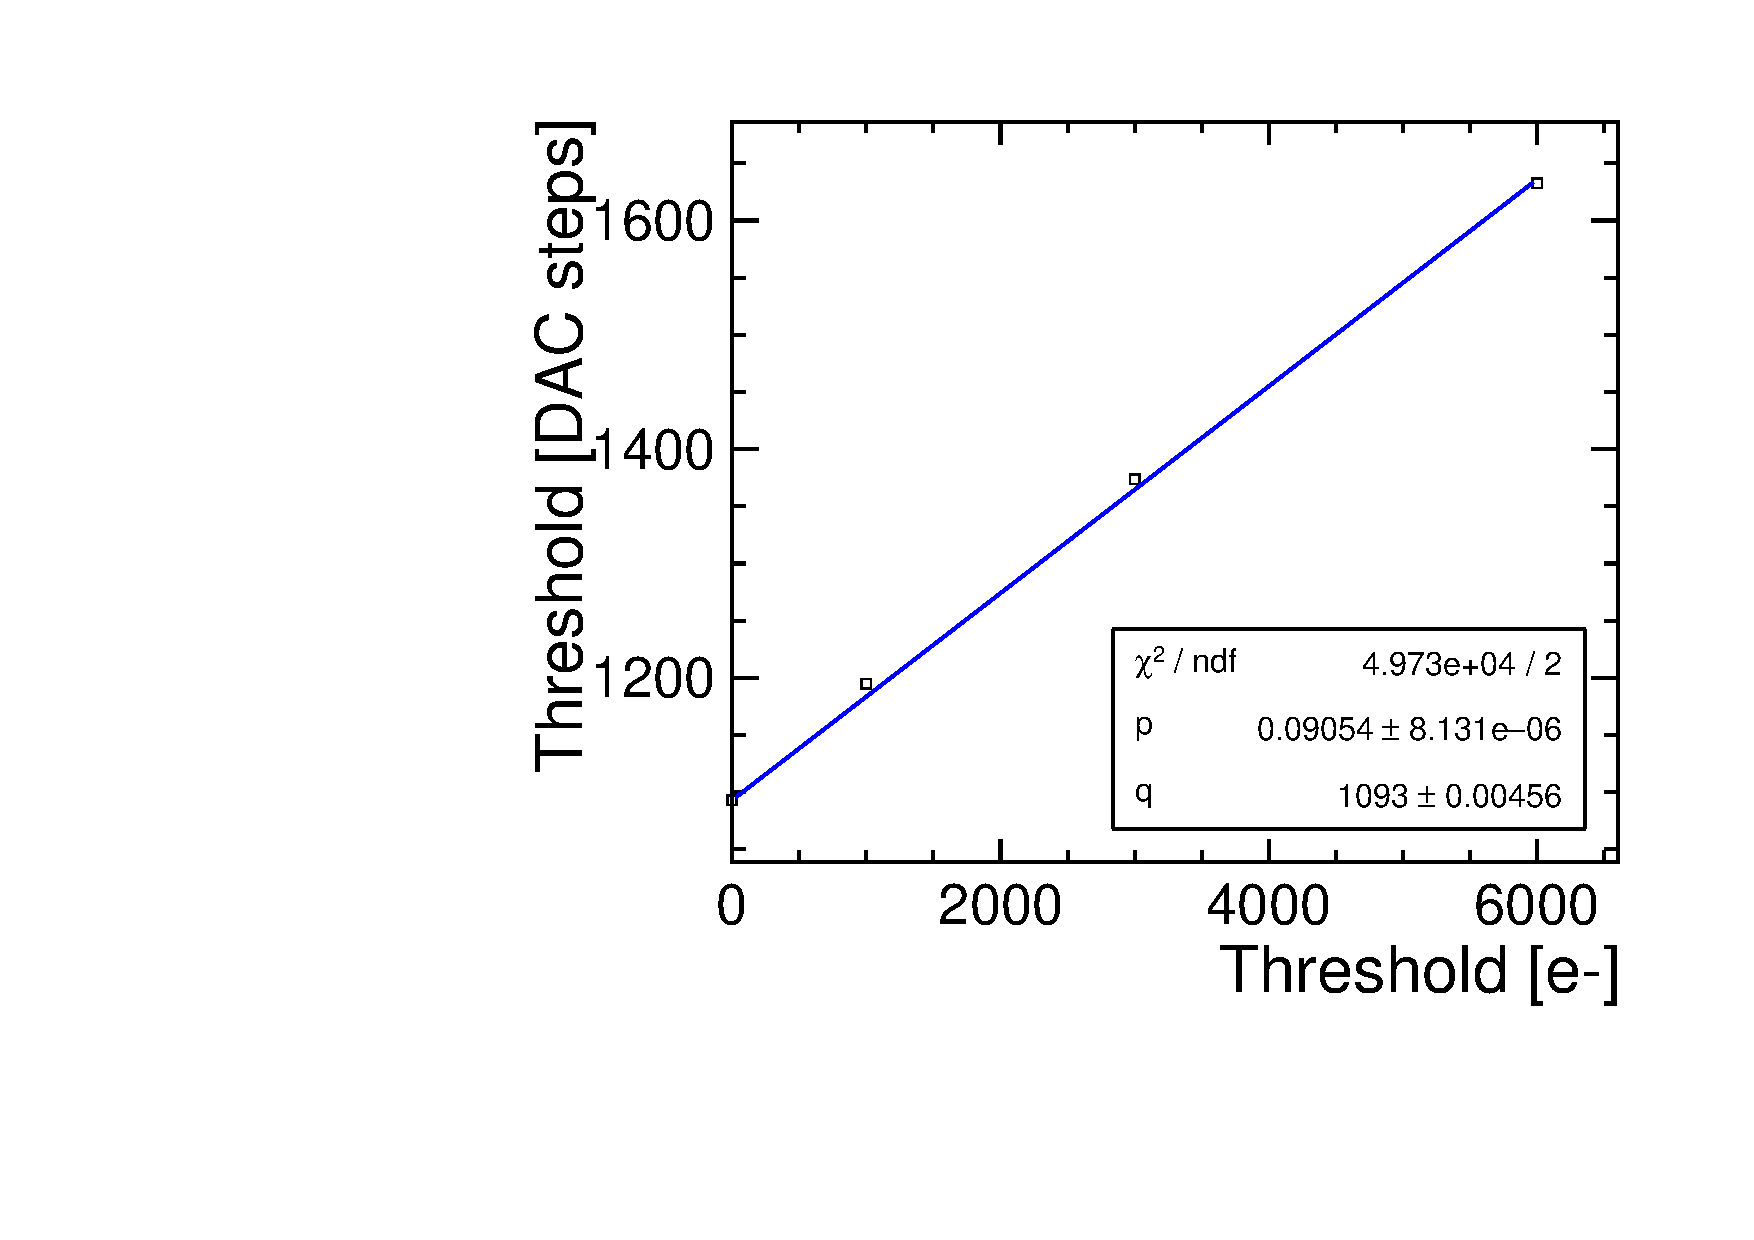
\includegraphics[width=0.9\textwidth]{./figures/Calibration/THLcalibration_W0019_C07.pdf}
    \caption{W19\_C7}
  \end{subfigure}\\
  \begin{subfigure}[b]{0.45\textwidth}
    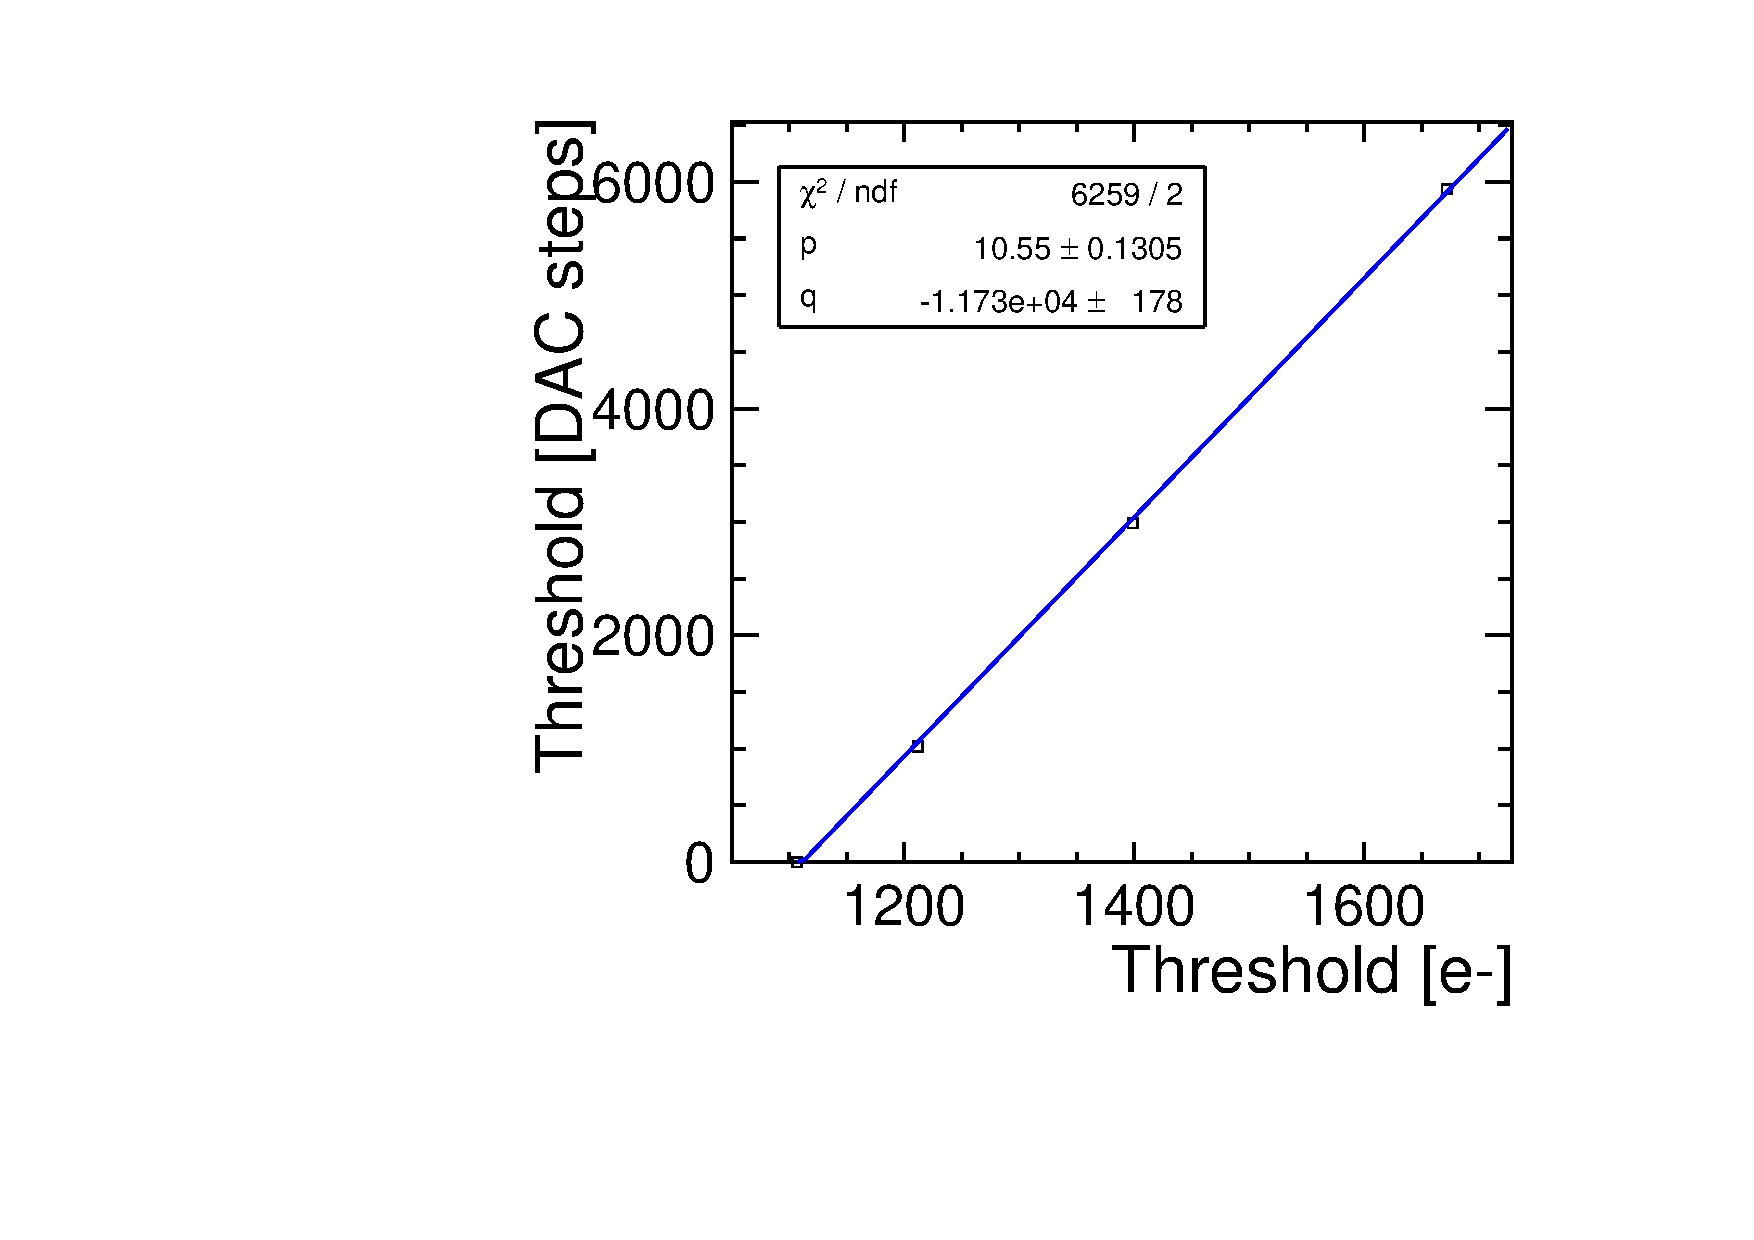
\includegraphics[width=0.9\textwidth]{./figures/Calibration/THLcalibration_W0005_E02.pdf}
    \caption{W5\_E2}
  \end{subfigure} \hfill
  \begin{subfigure}[b]{0.45\textwidth}
    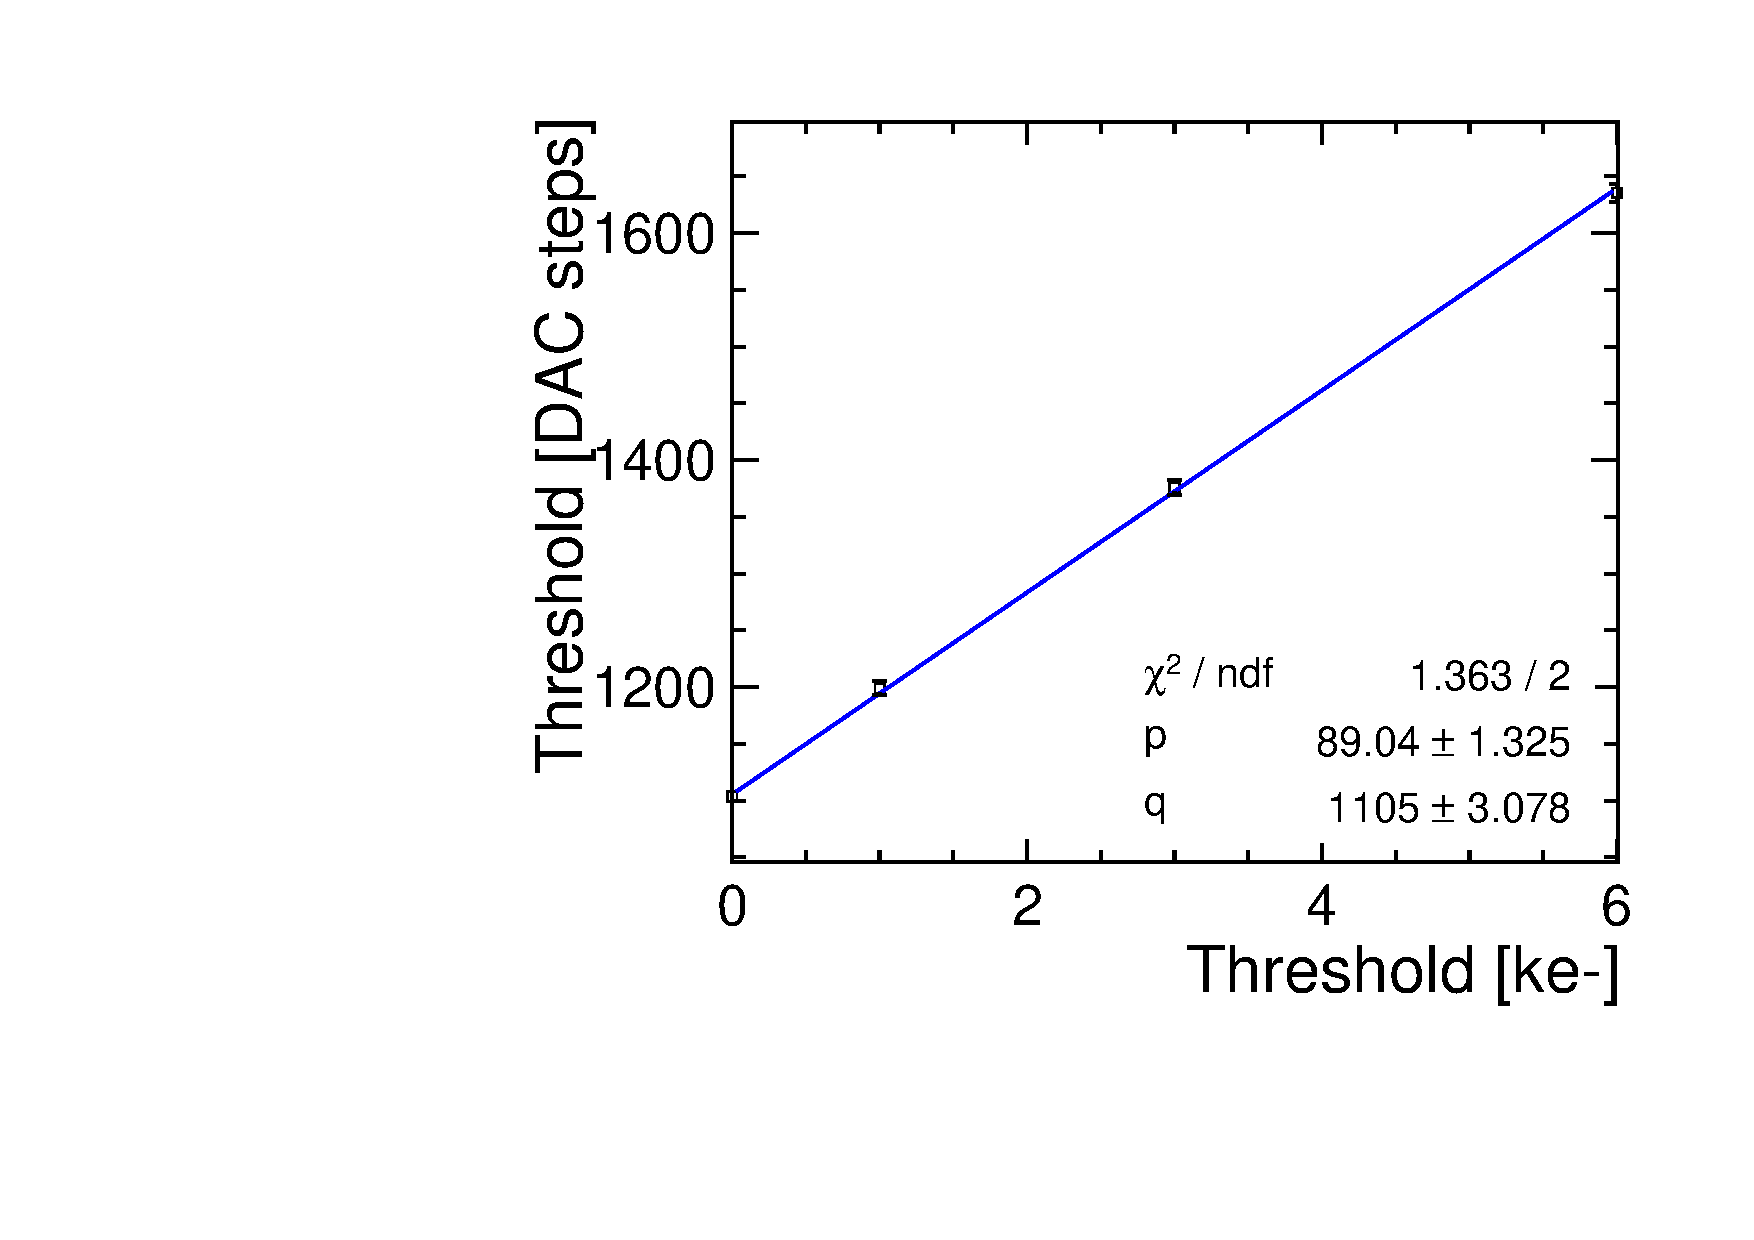
\includegraphics[width=0.9\textwidth]{./figures/Calibration/THLcalibration_W0005_F01.pdf}
    \caption{W5\_F1}
  \end{subfigure}%\\
  %% \begin{subfigure}[b]{0.45\textwidth}
  %%   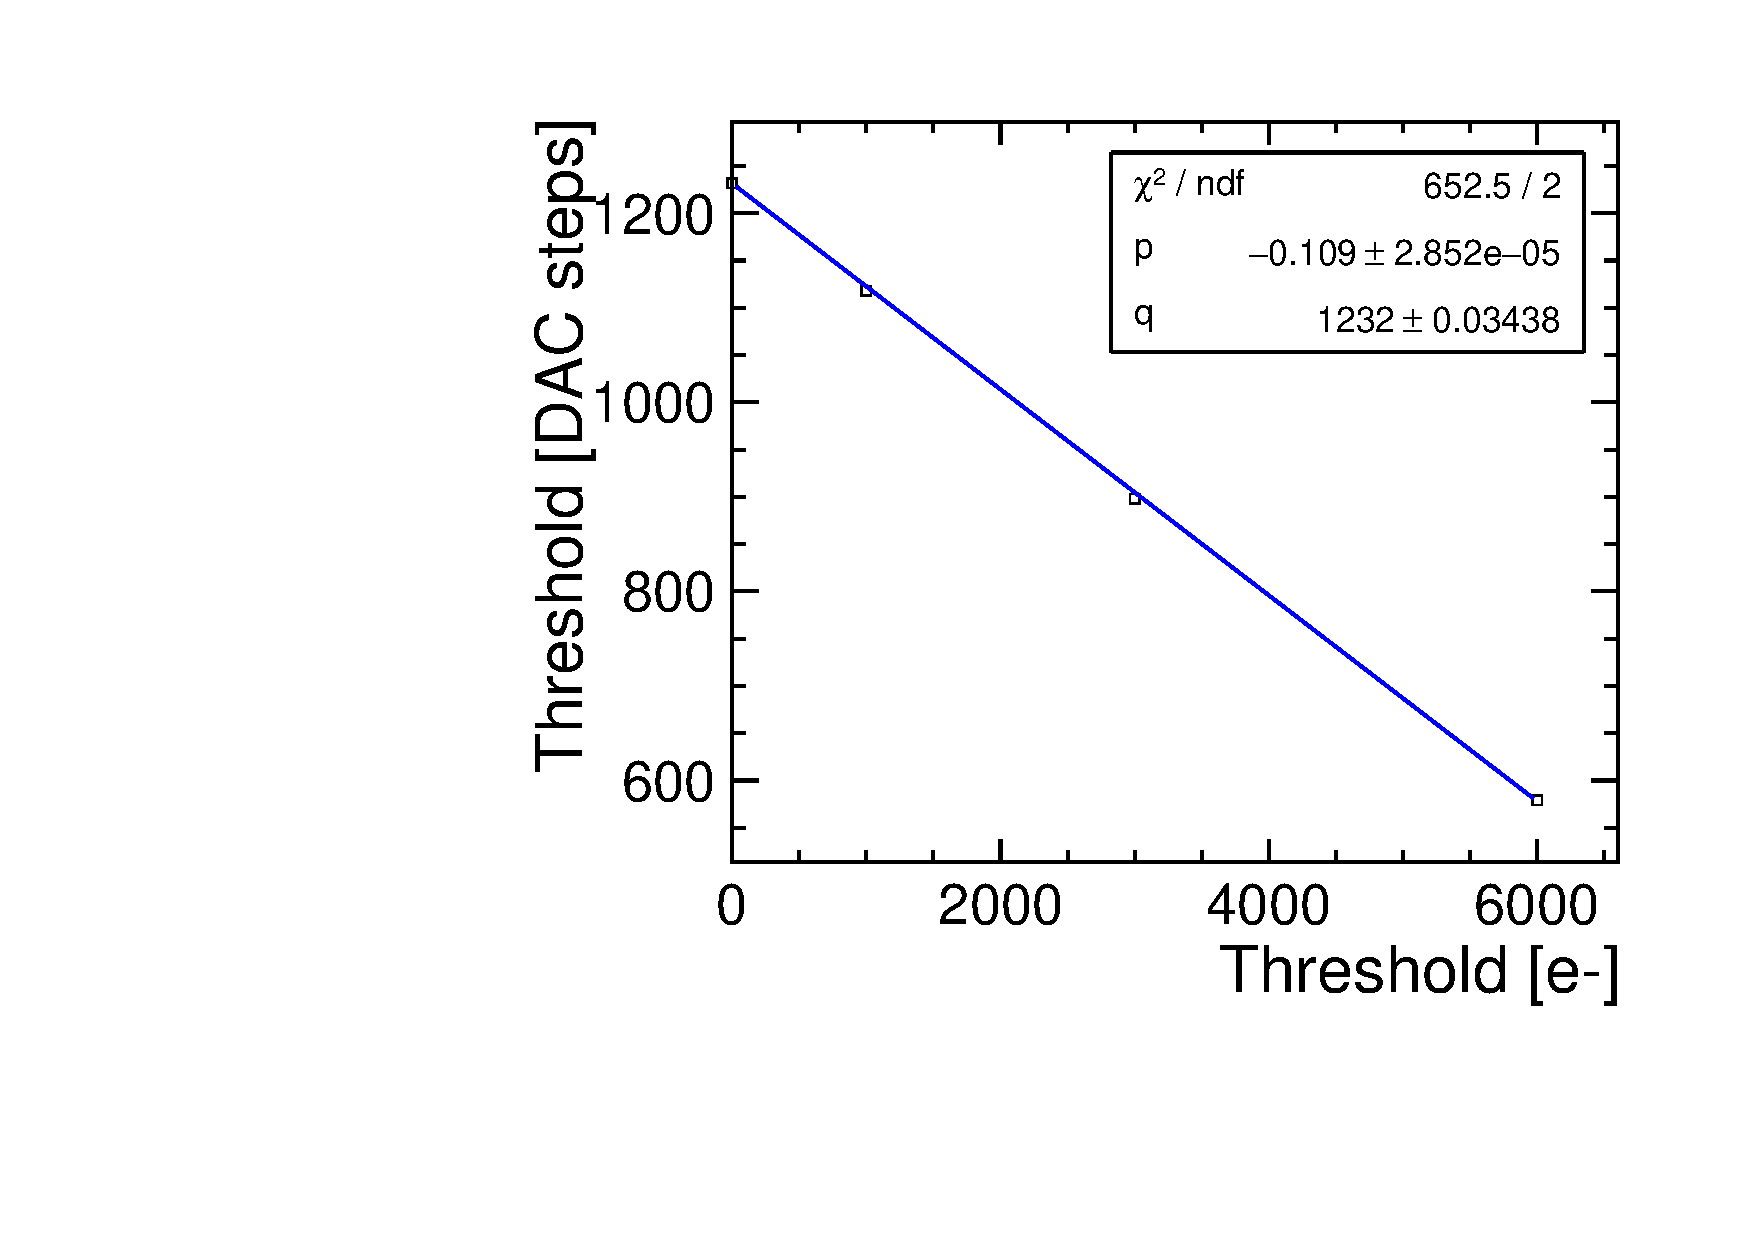
\includegraphics[width=0.9\textwidth]{./figures/Calibration/THLcalibration_W0002_J05.pdf}
  %%   \caption{W0002\_J05}
  %% \end{subfigure}
  \caption{Threshold calibration for the assemblies listed in
    \cref{tab:Timepix3Assemblies}. Each point corresponds to the
    maximum gradient of the S-curve for each pulse height. A linear
    function as described in \cref{eq:THLDAC} was used to fit the data
    points and obtain the parameters $p$ and $q$.}
  \label{fig:Timepix3_THL_Calibration}
\end{figure}


% \section{Application of the calibration to the test-beam data}\label{sec:appendixCalibDataG4}


% \begin{figure}[htbp] \centering
%   \begin{subfigure}[b]{0.32\textwidth}
%     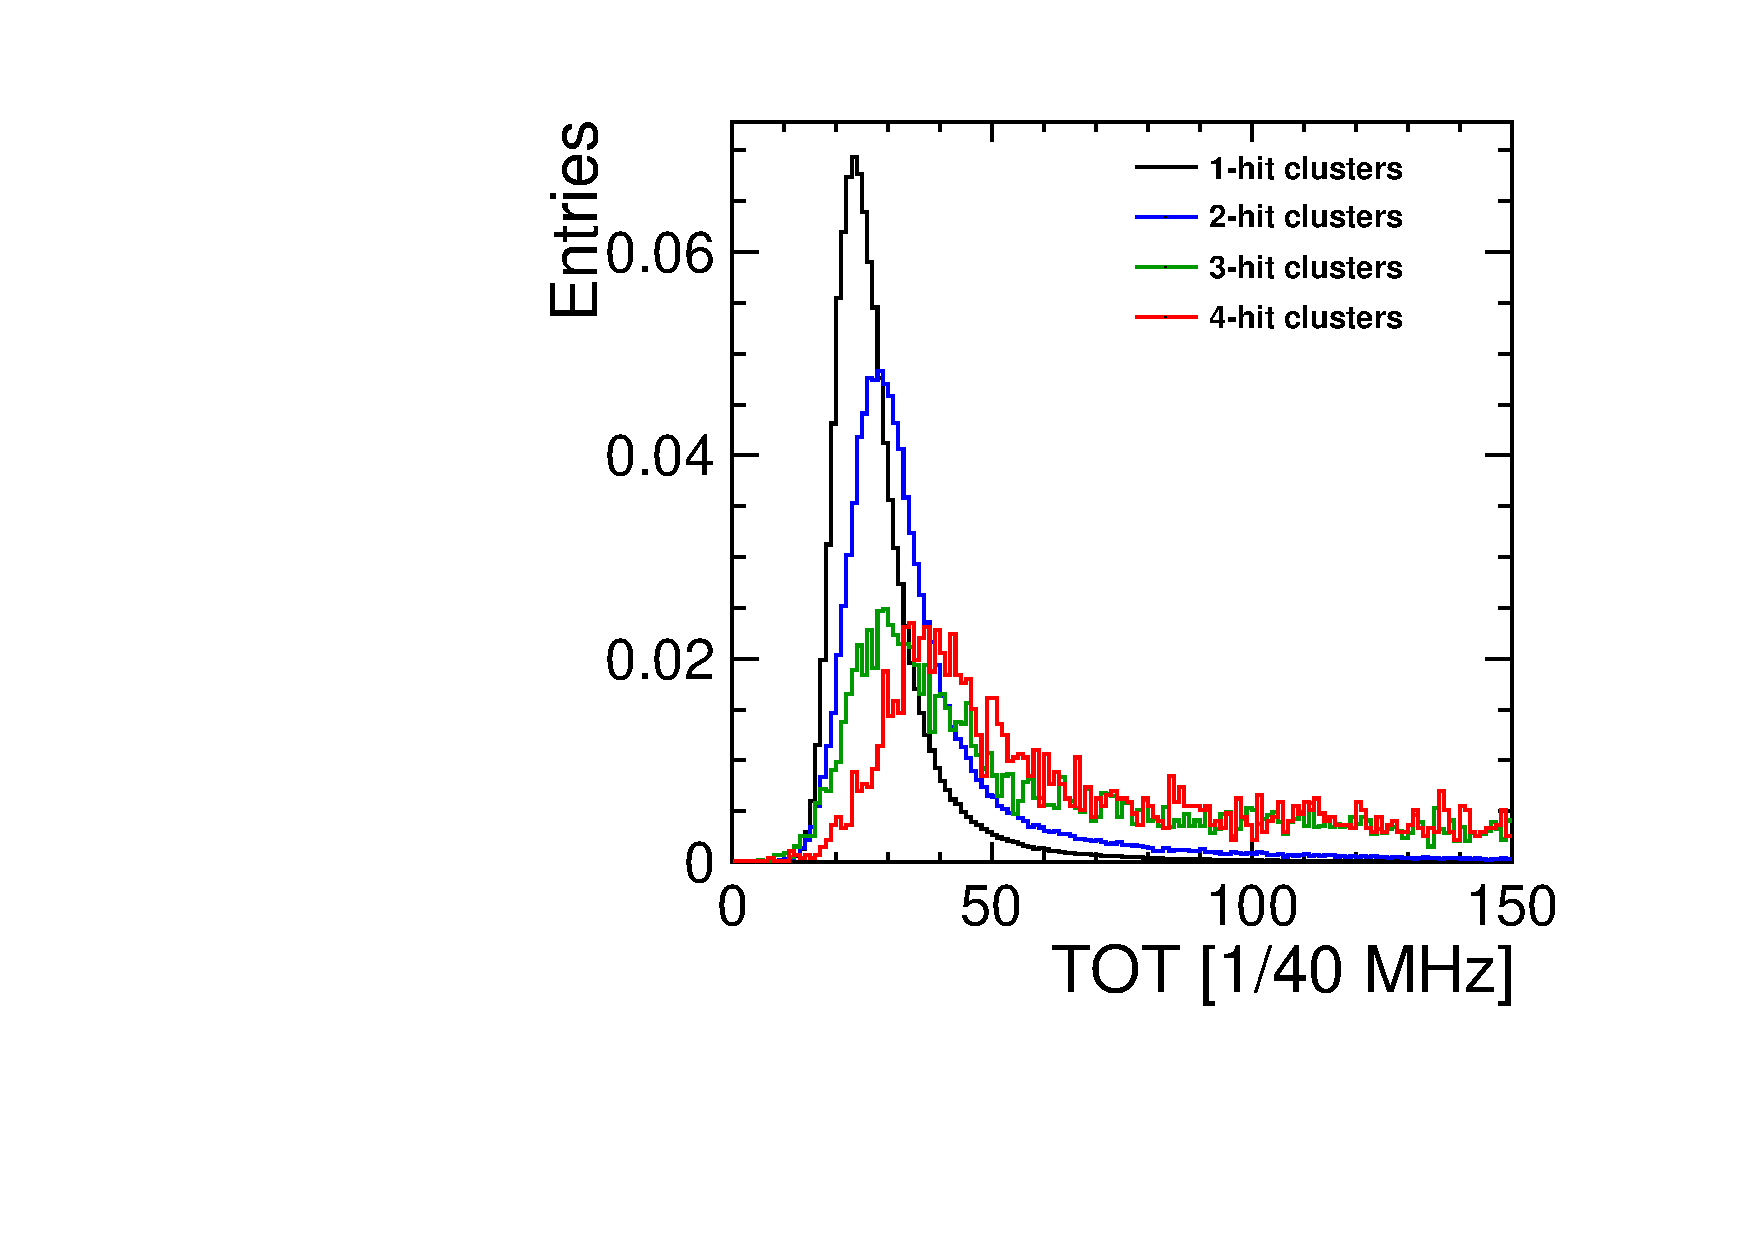
\includegraphics[width=\textwidth]{./figures/Calibration/TOT_Clusters_W0019_G07.pdf}
%     \caption{}
%   \end{subfigure}\hfill
%   \begin{subfigure}[b]{0.32\textwidth}
%     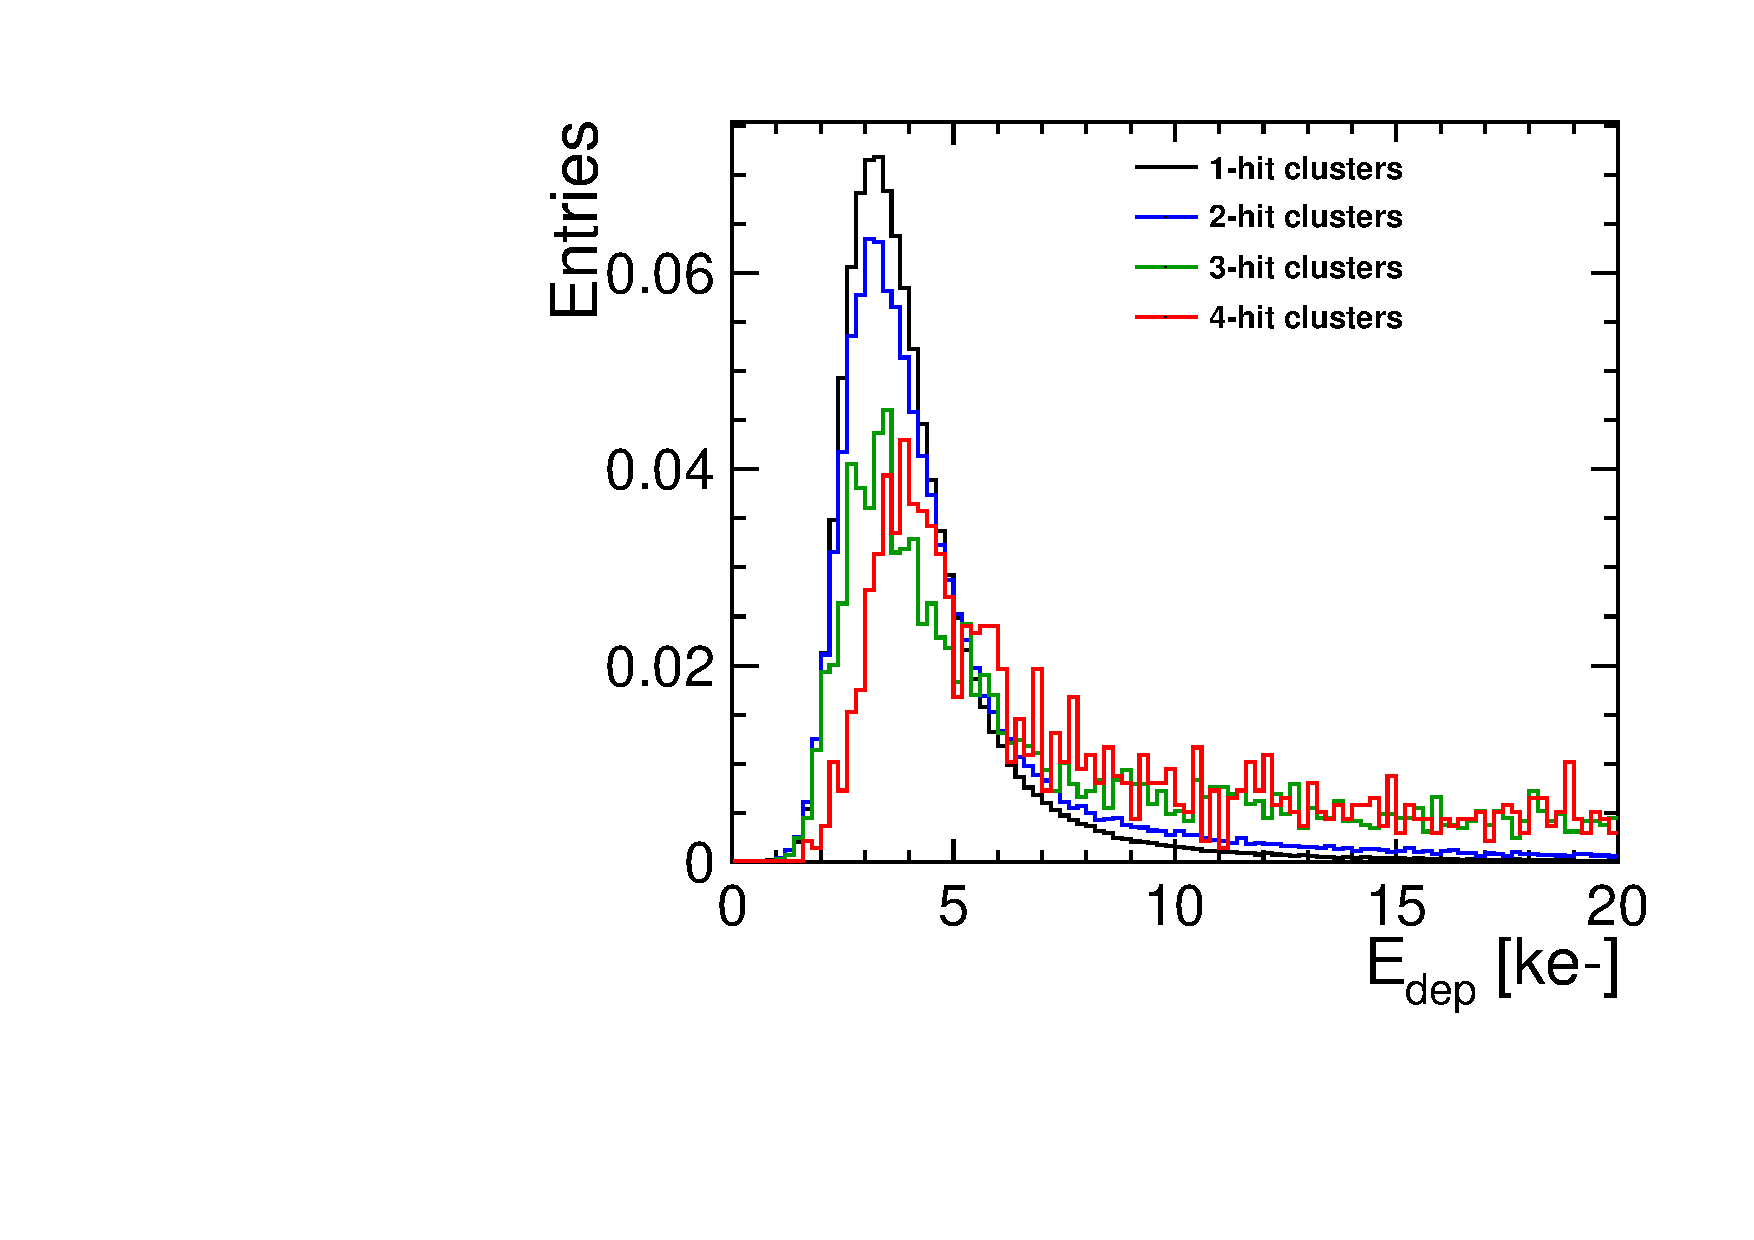
\includegraphics[width=\textwidth]{./figures/Calibration/Edep_Clusters_W0019_G07.pdf}
%     \caption{}
%   \end{subfigure}\hfill
%   \begin{subfigure}[b]{0.32\textwidth}
%     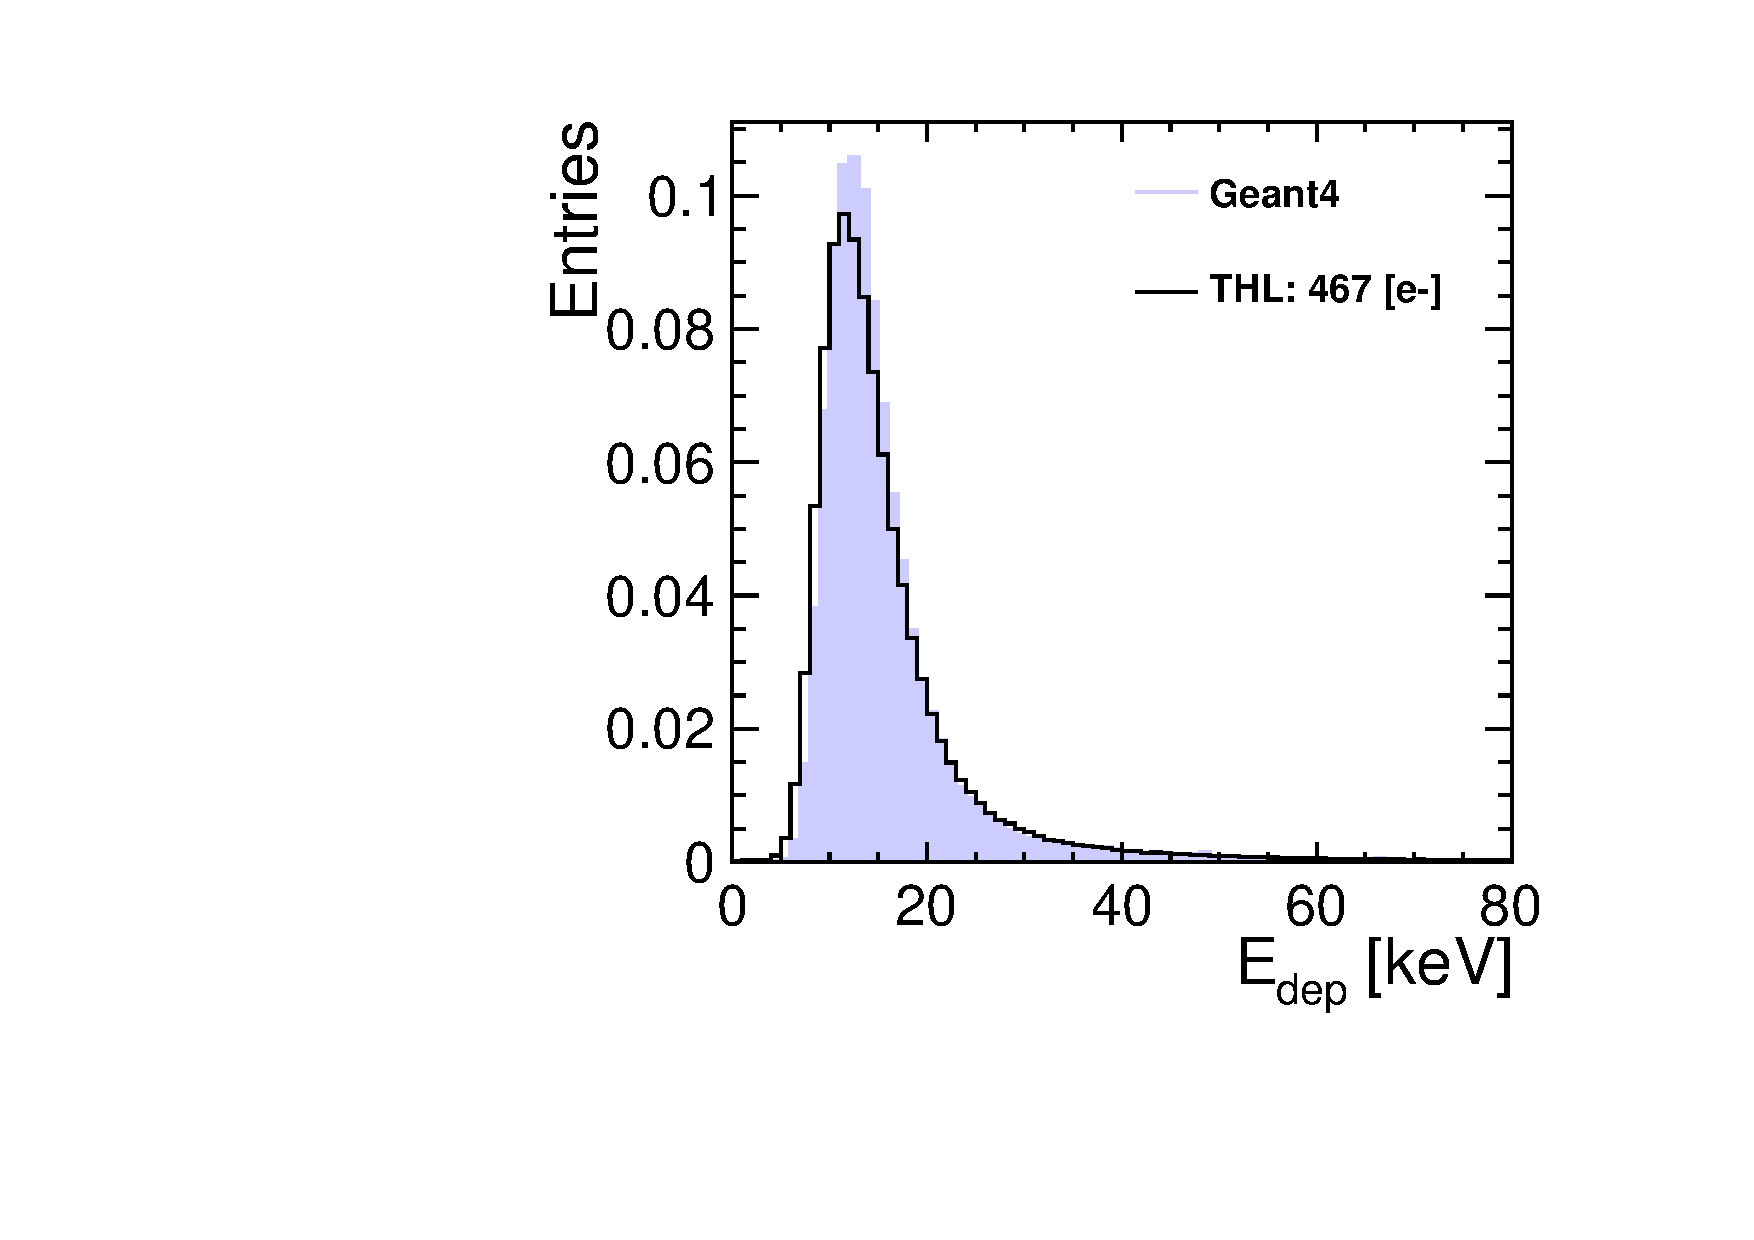
\includegraphics[width=\textwidth]{./figures/Calibration/Edep_G4_W0019_G07.pdf}
%     \caption{}
%   \end{subfigure}
%   \caption{Energy deposition and comparison to
%     \textsc{Geant4}. W0019\_G07, Run 1190, THL=995.}
%   \label{fig:EdepW19L8}
% \end{figure}


% \begin{figure}[htbp] \centering
%   \begin{subfigure}[b]{0.32\textwidth}
%     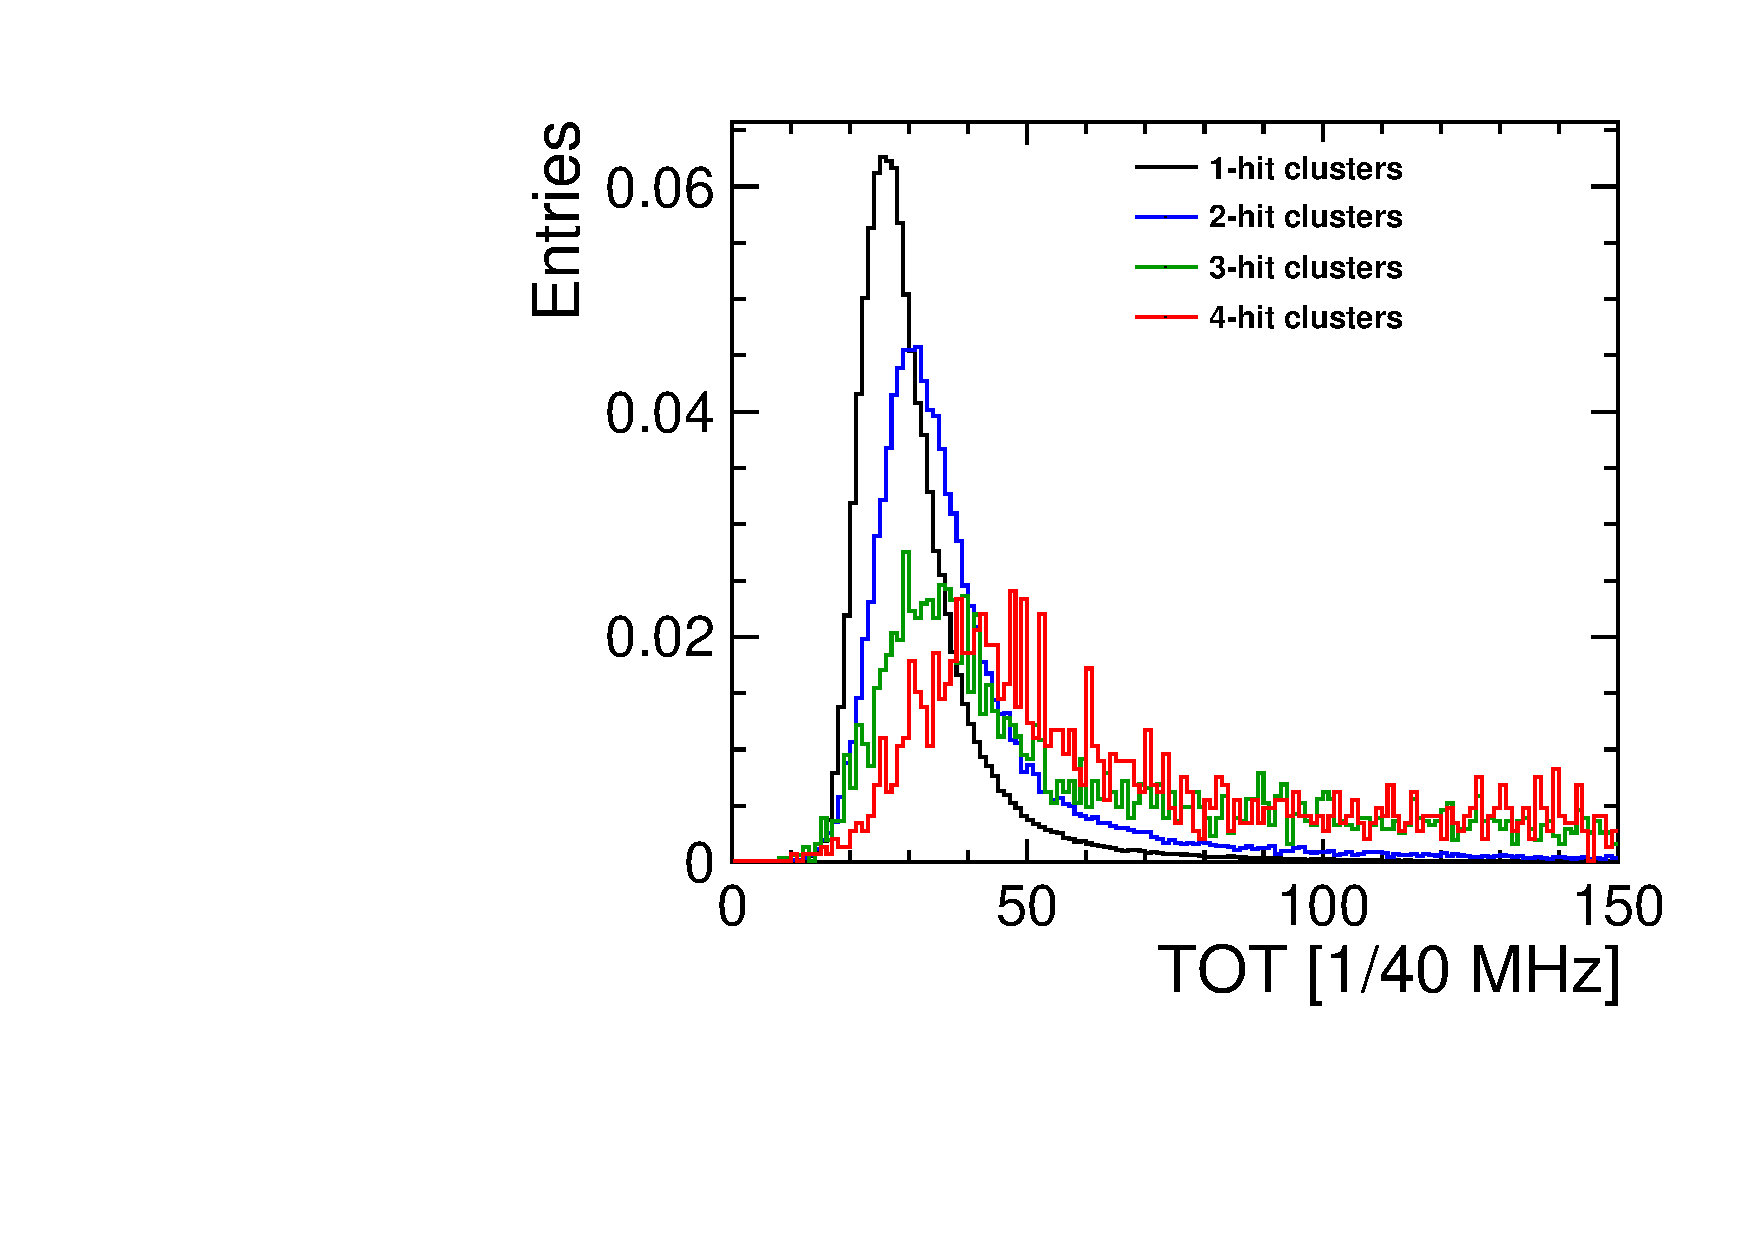
\includegraphics[width=\textwidth]{./figures/Calibration/TOT_Clusters_W0019_F07.pdf}
%     \caption{}
%   \end{subfigure}\hfill
%   \begin{subfigure}[b]{0.32\textwidth}
%     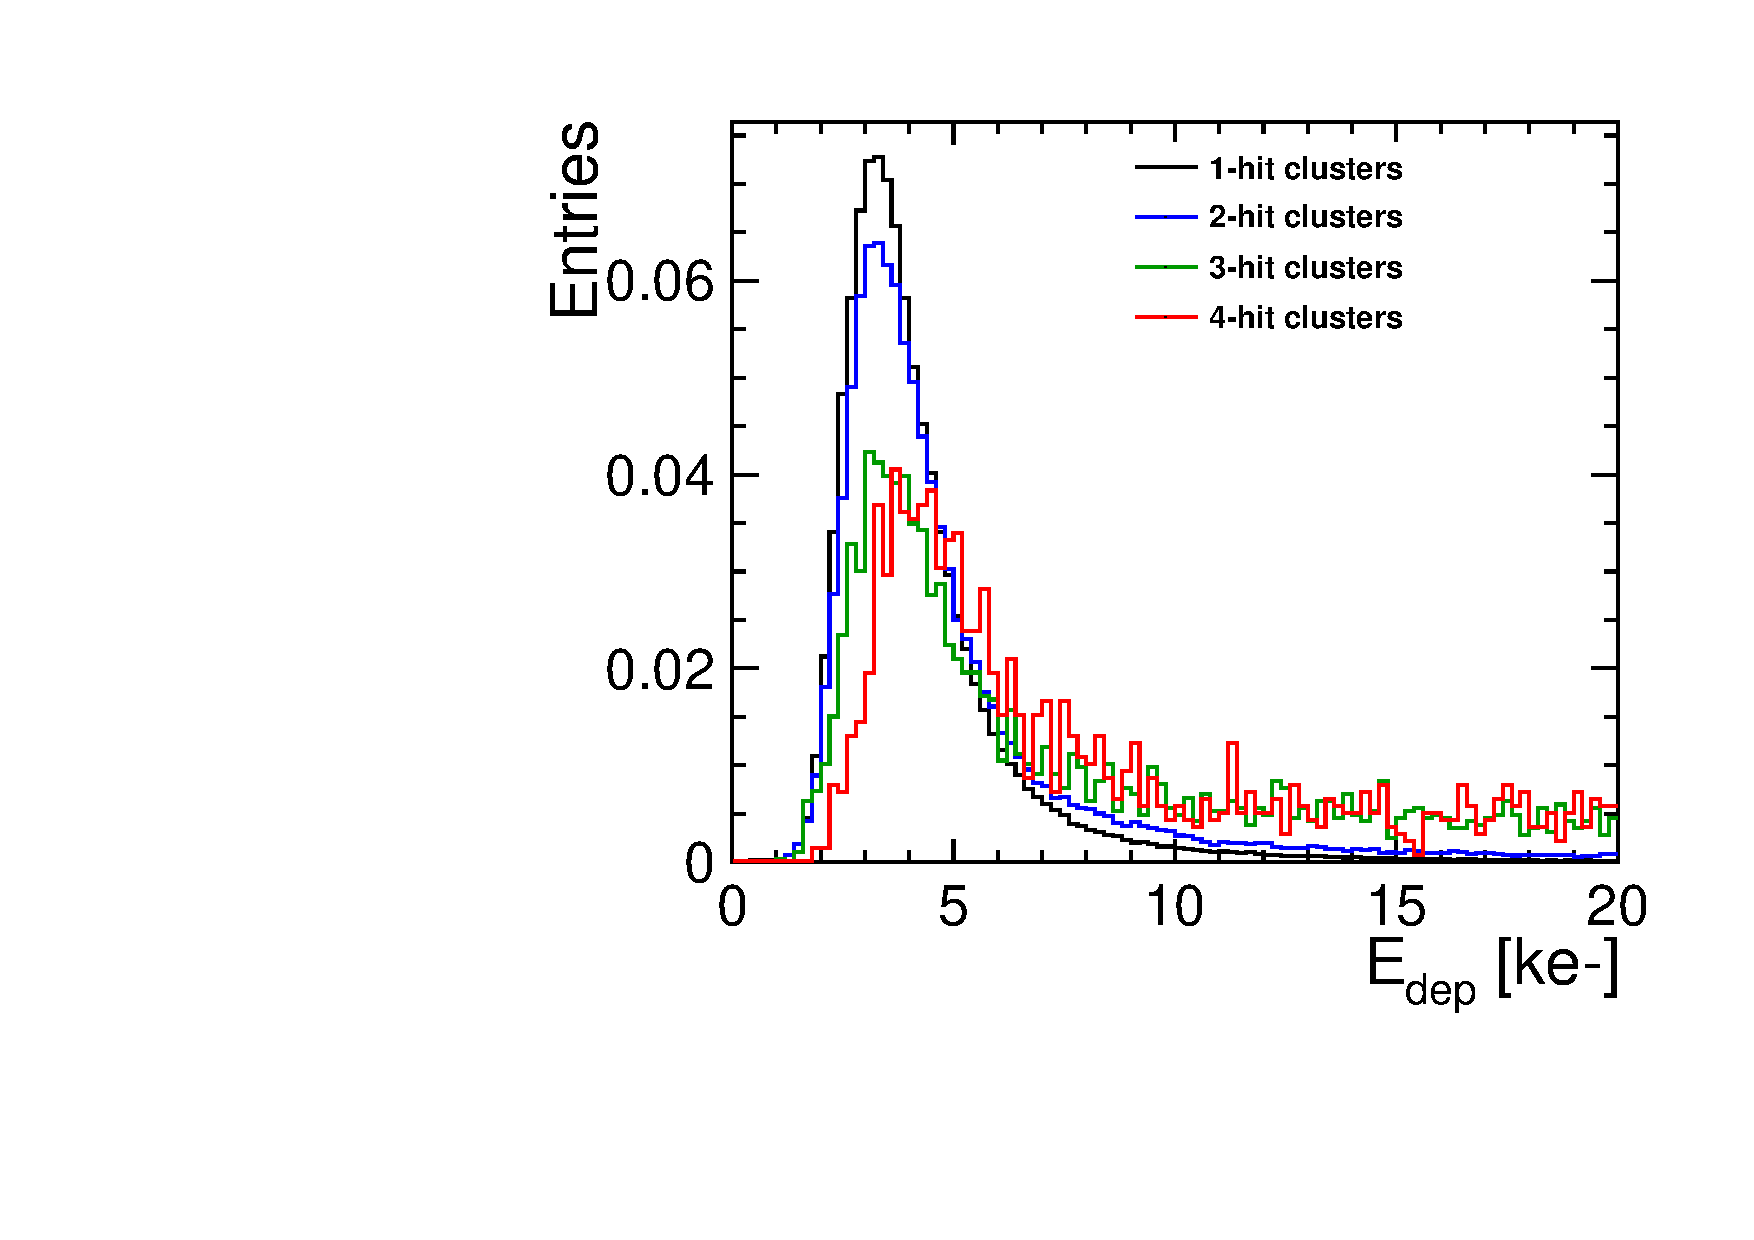
\includegraphics[width=\textwidth]{./figures/Calibration/Edep_Clusters_W0019_F07.pdf}
%     \caption{}
%   \end{subfigure}\hfill
%   \begin{subfigure}[b]{0.32\textwidth}
% %    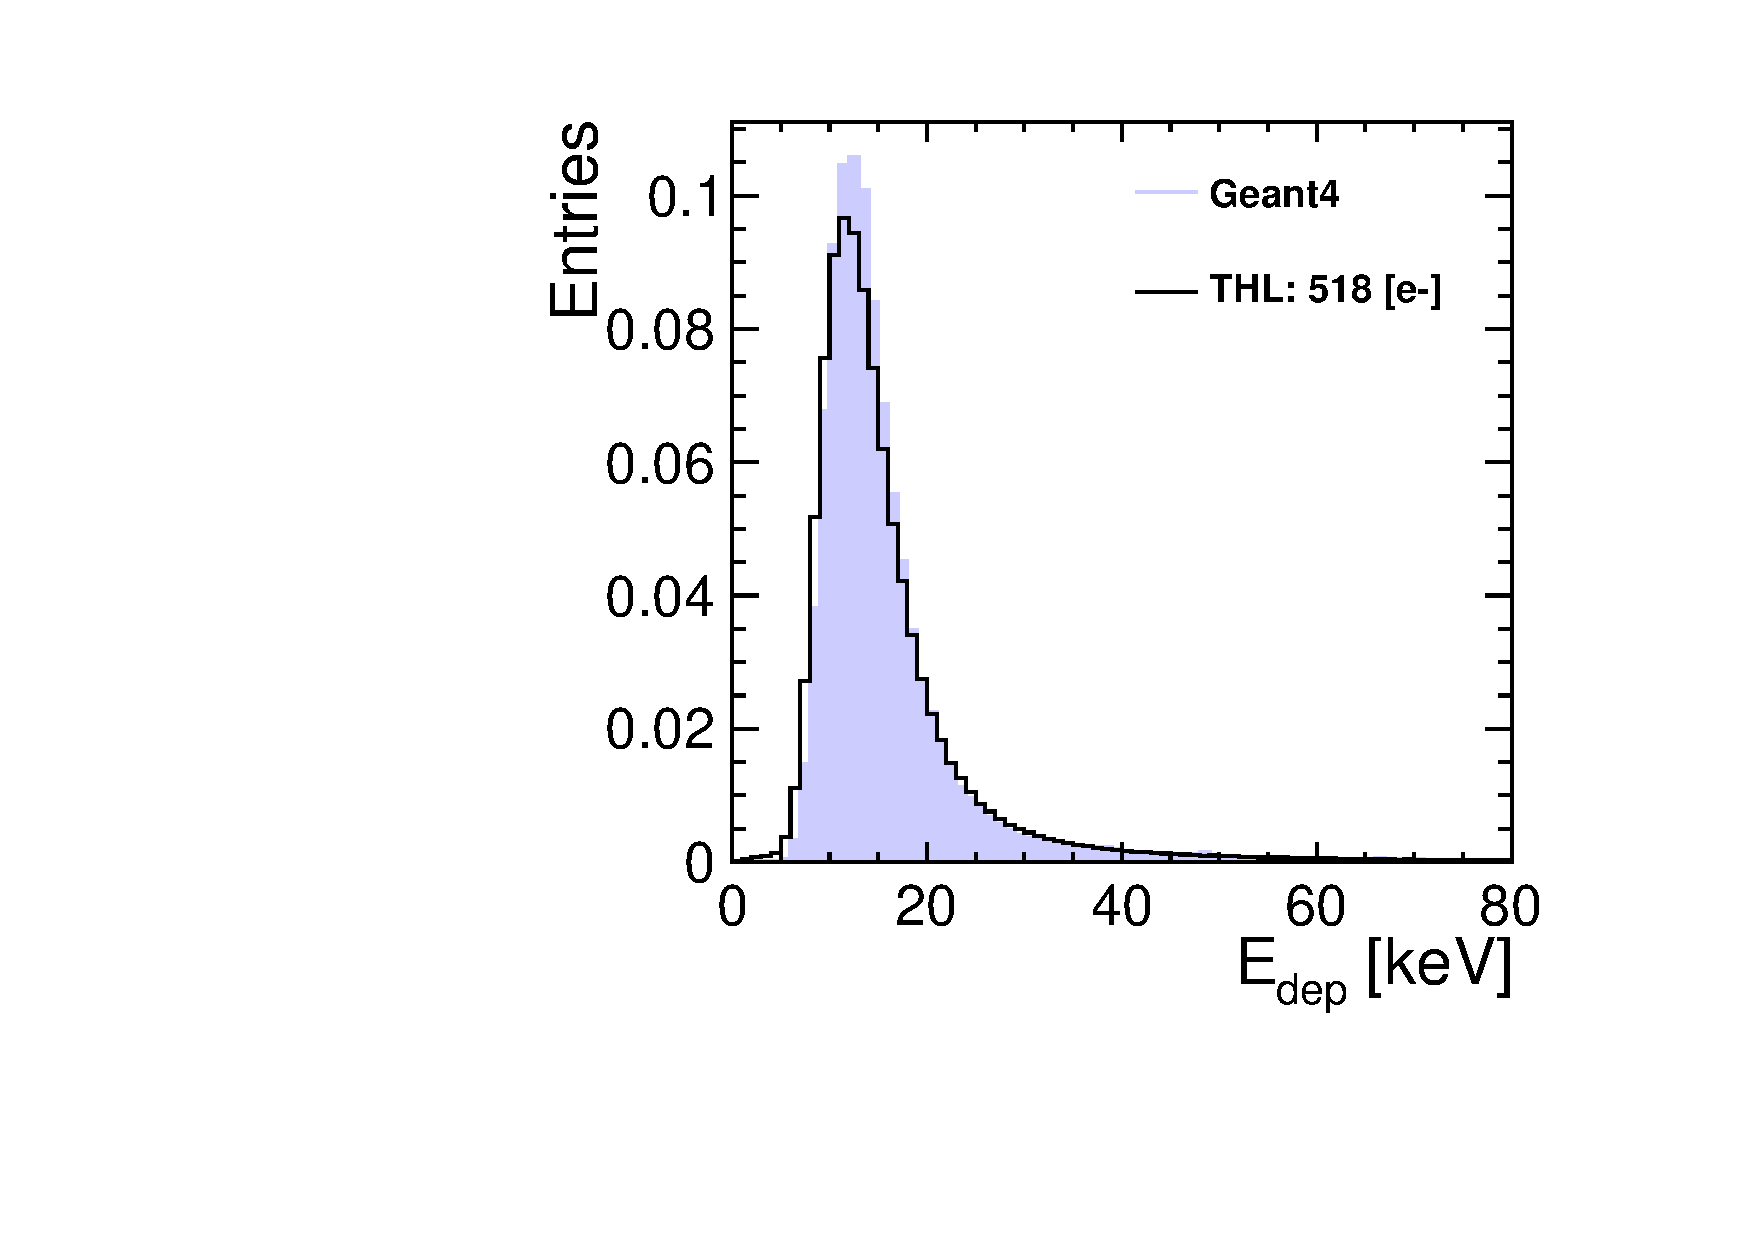
\includegraphics[width=\textwidth]{./figures/Calibration/Edep_G4_W0019_L08.pdf}
%     \caption{}
%   \end{subfigure}
%   \caption{Energy deposition and comparison to
%     \textsc{Geant4}. W0019\_L08, Run 1130, THL=1133.}
%   \label{fig:EdepW19L8}
% \end{figure}


% \begin{figure}[htbp] \centering
%   \begin{subfigure}[b]{0.32\textwidth}
%     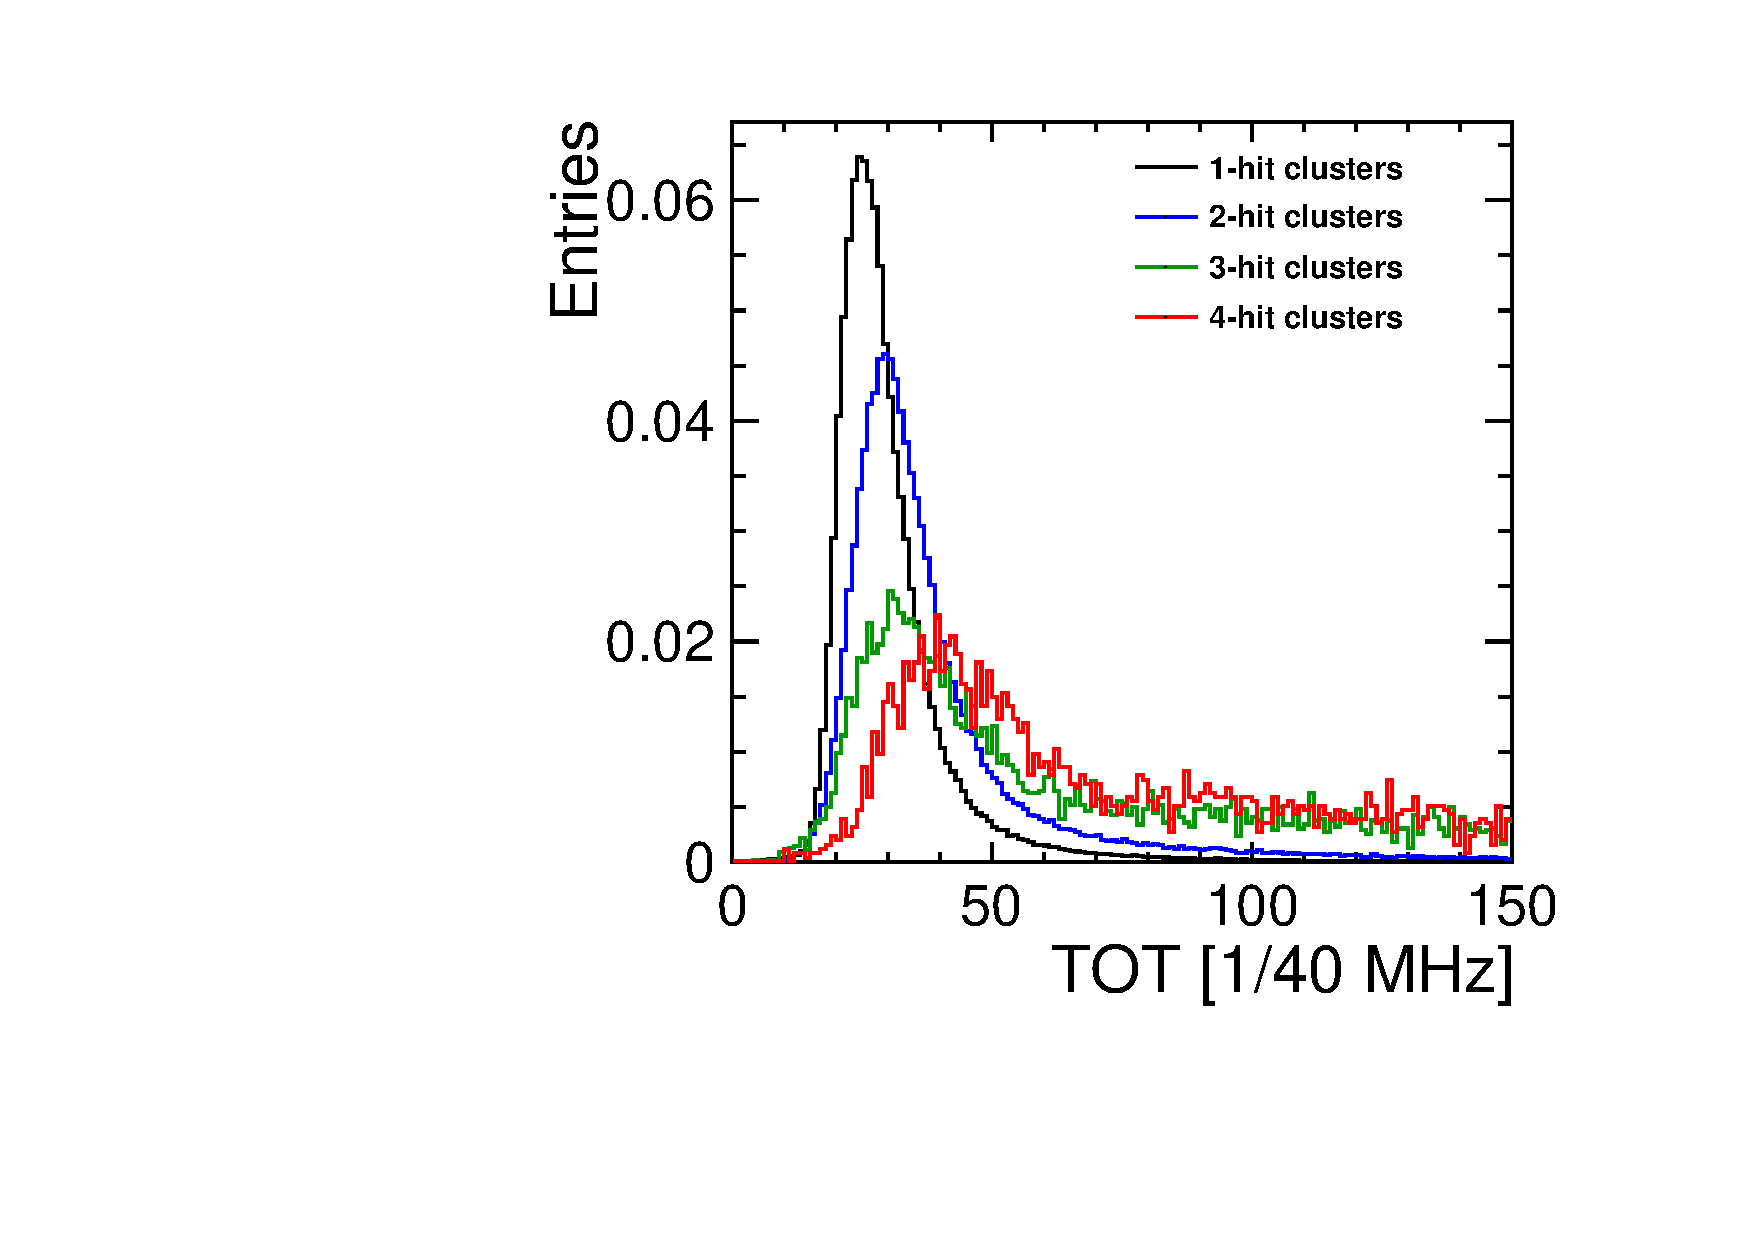
\includegraphics[width=\textwidth]{./figures/Calibration/TOT_Clusters_W0019_L08.pdf}
%     \caption{}
%   \end{subfigure}\hfill
%   \begin{subfigure}[b]{0.32\textwidth}
%     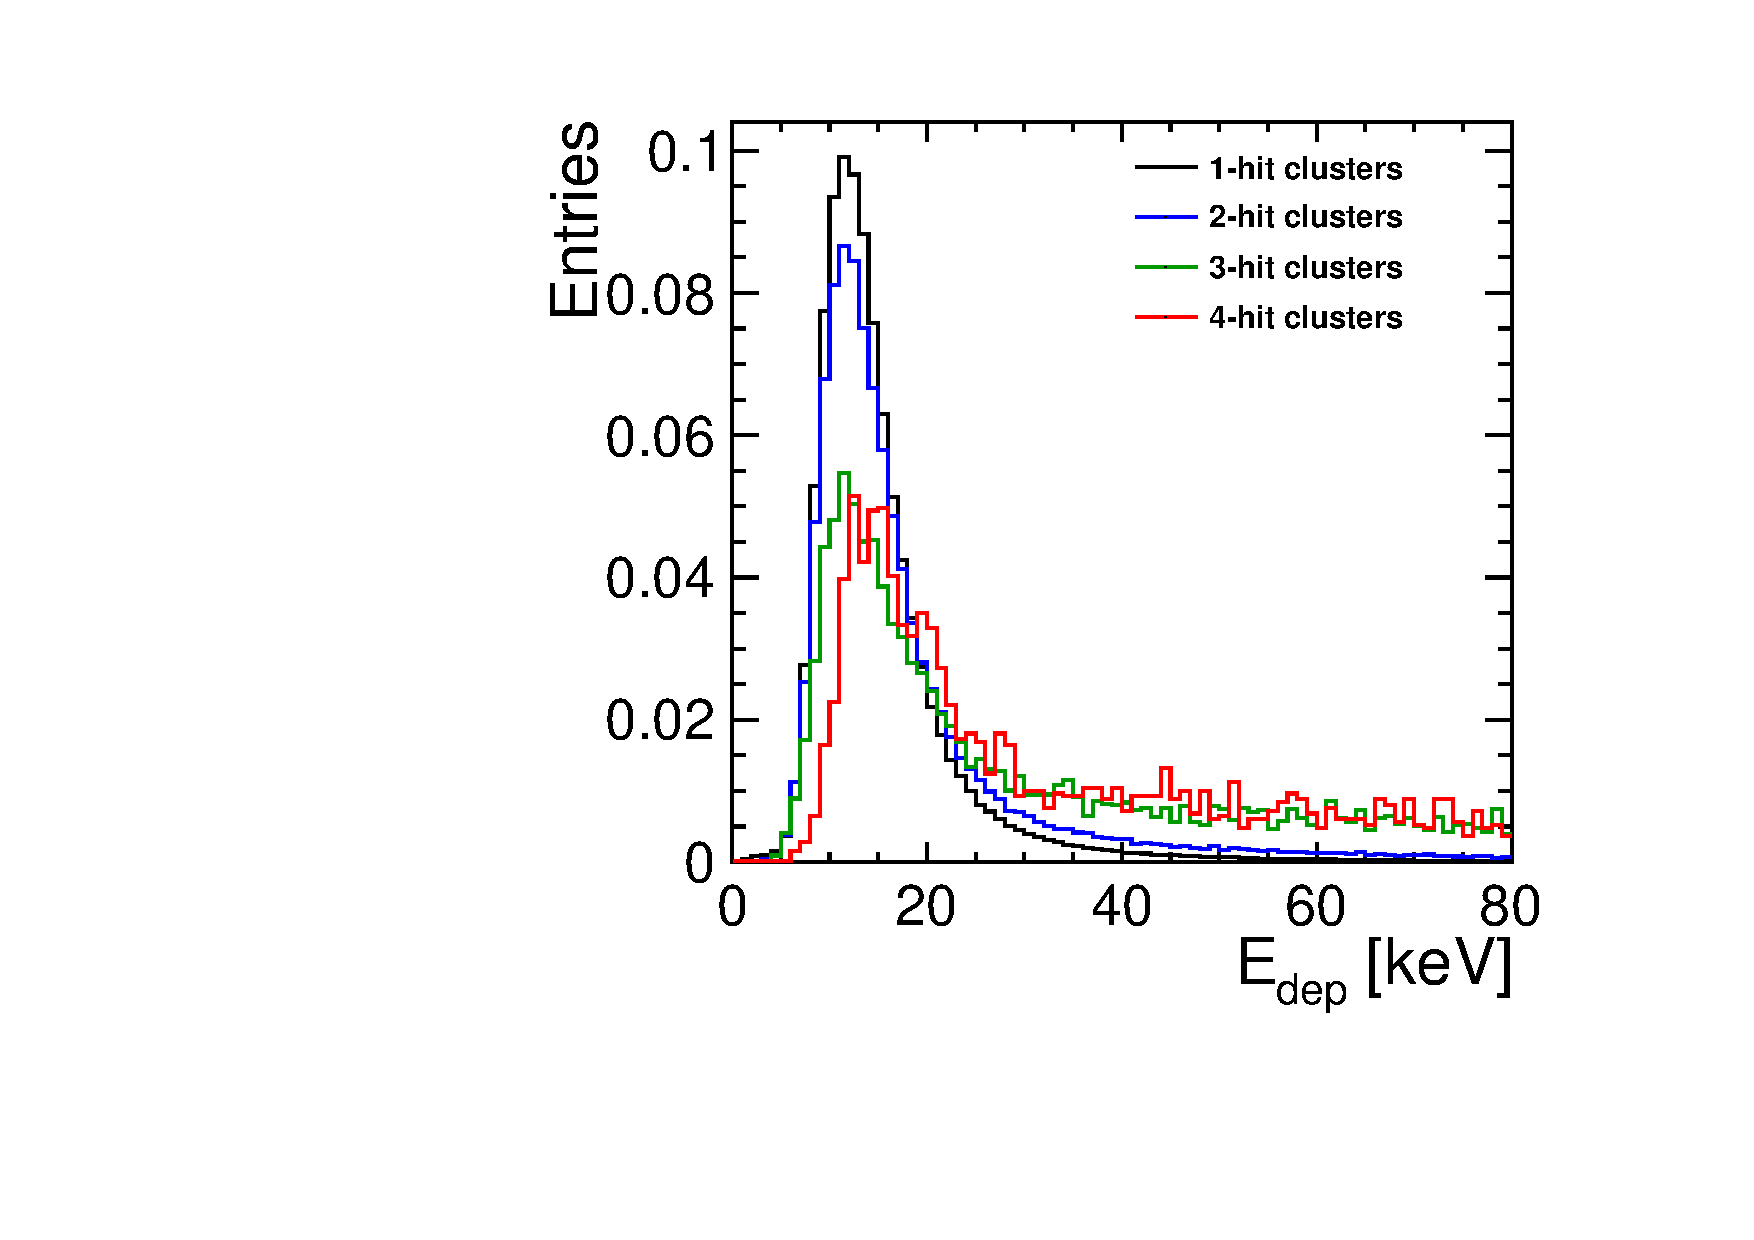
\includegraphics[width=\textwidth]{./figures/Calibration/Edep_Clusters_W0019_L08.pdf}
%     \caption{}
%   \end{subfigure}\hfill
%   \begin{subfigure}[b]{0.32\textwidth}
%     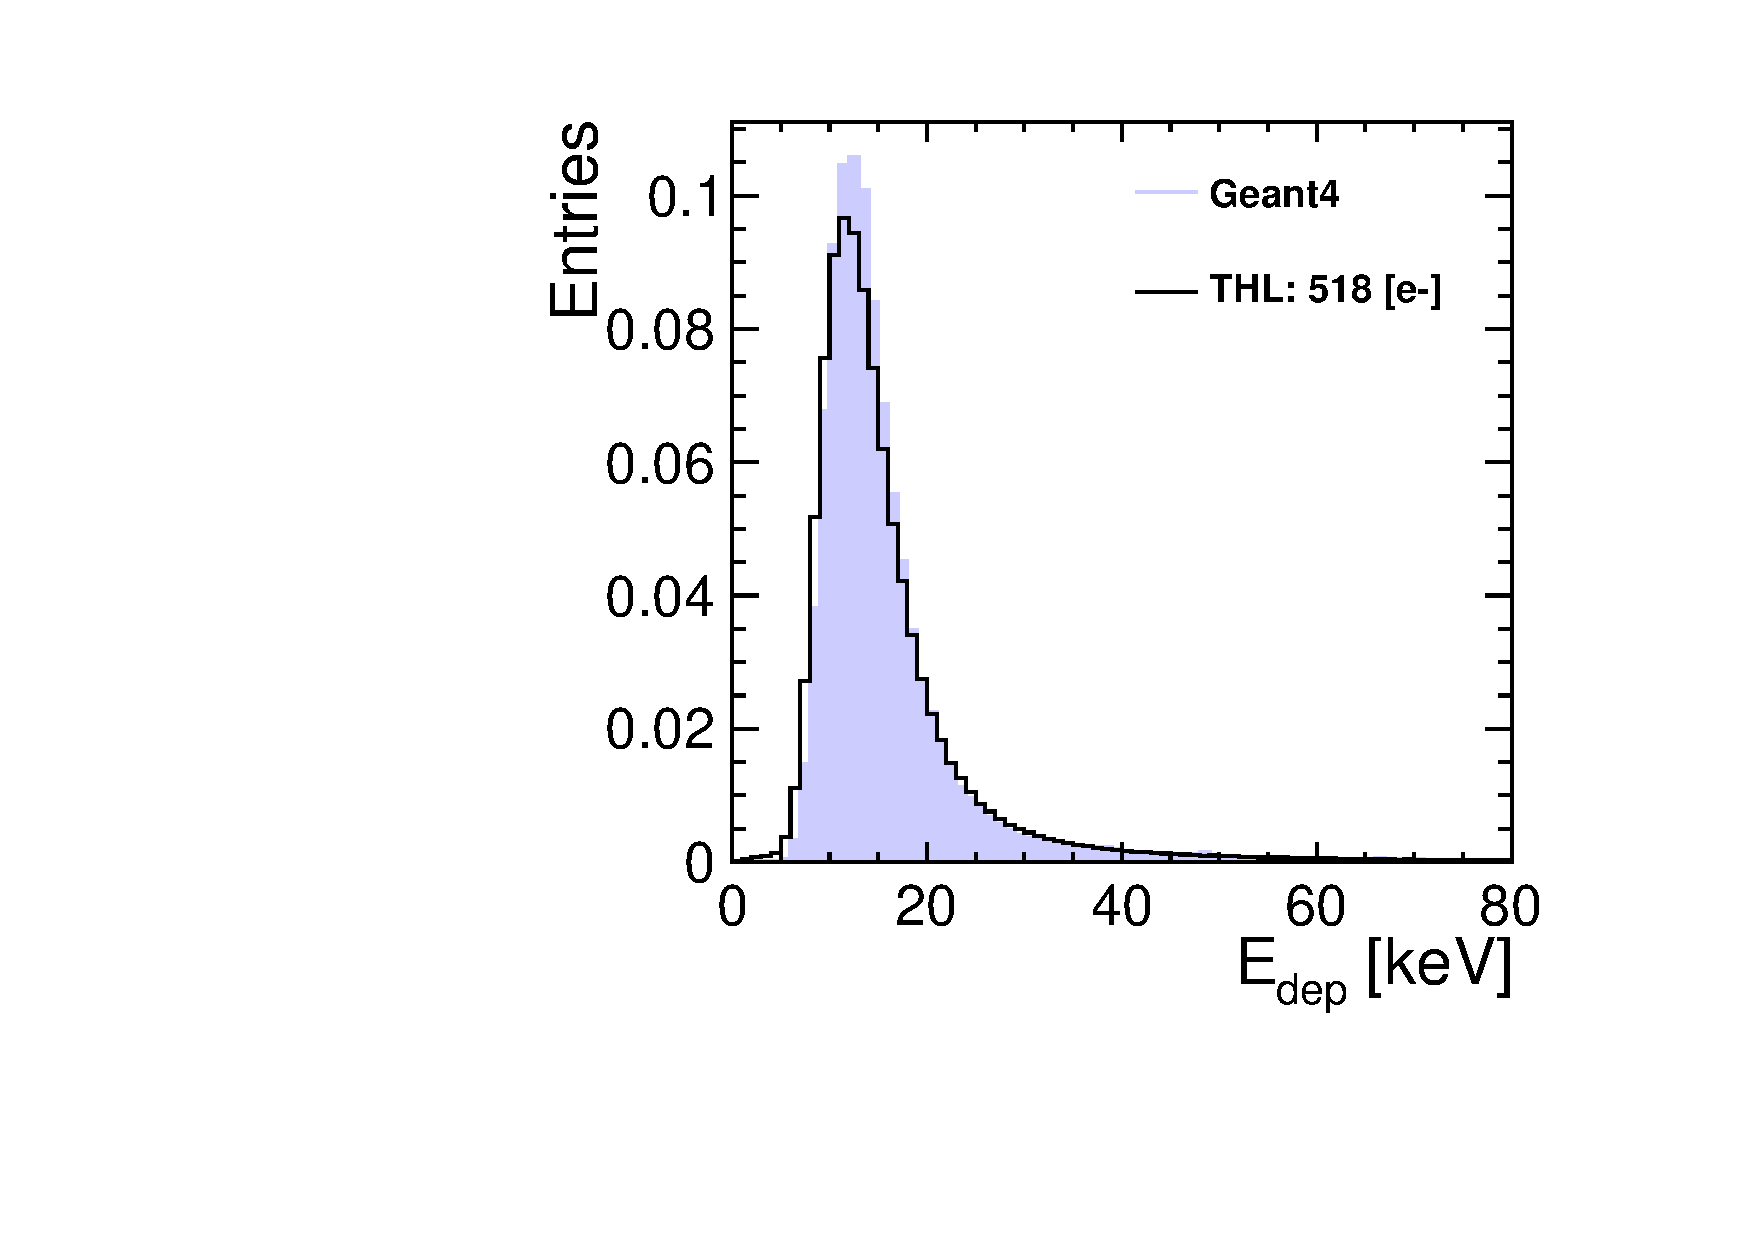
\includegraphics[width=\textwidth]{./figures/Calibration/Edep_G4_W0019_L08.pdf}
%     \caption{}
%   \end{subfigure}
%   \caption{Energy deposition and comparison to
%     \textsc{Geant4}. W0019\_L08, Run 1130, THL=1133.}
%   \label{fig:EdepW19L8}
% \end{figure}


% \begin{figure}[htbp] \centering
%   \begin{subfigure}[b]{0.32\textwidth}
%     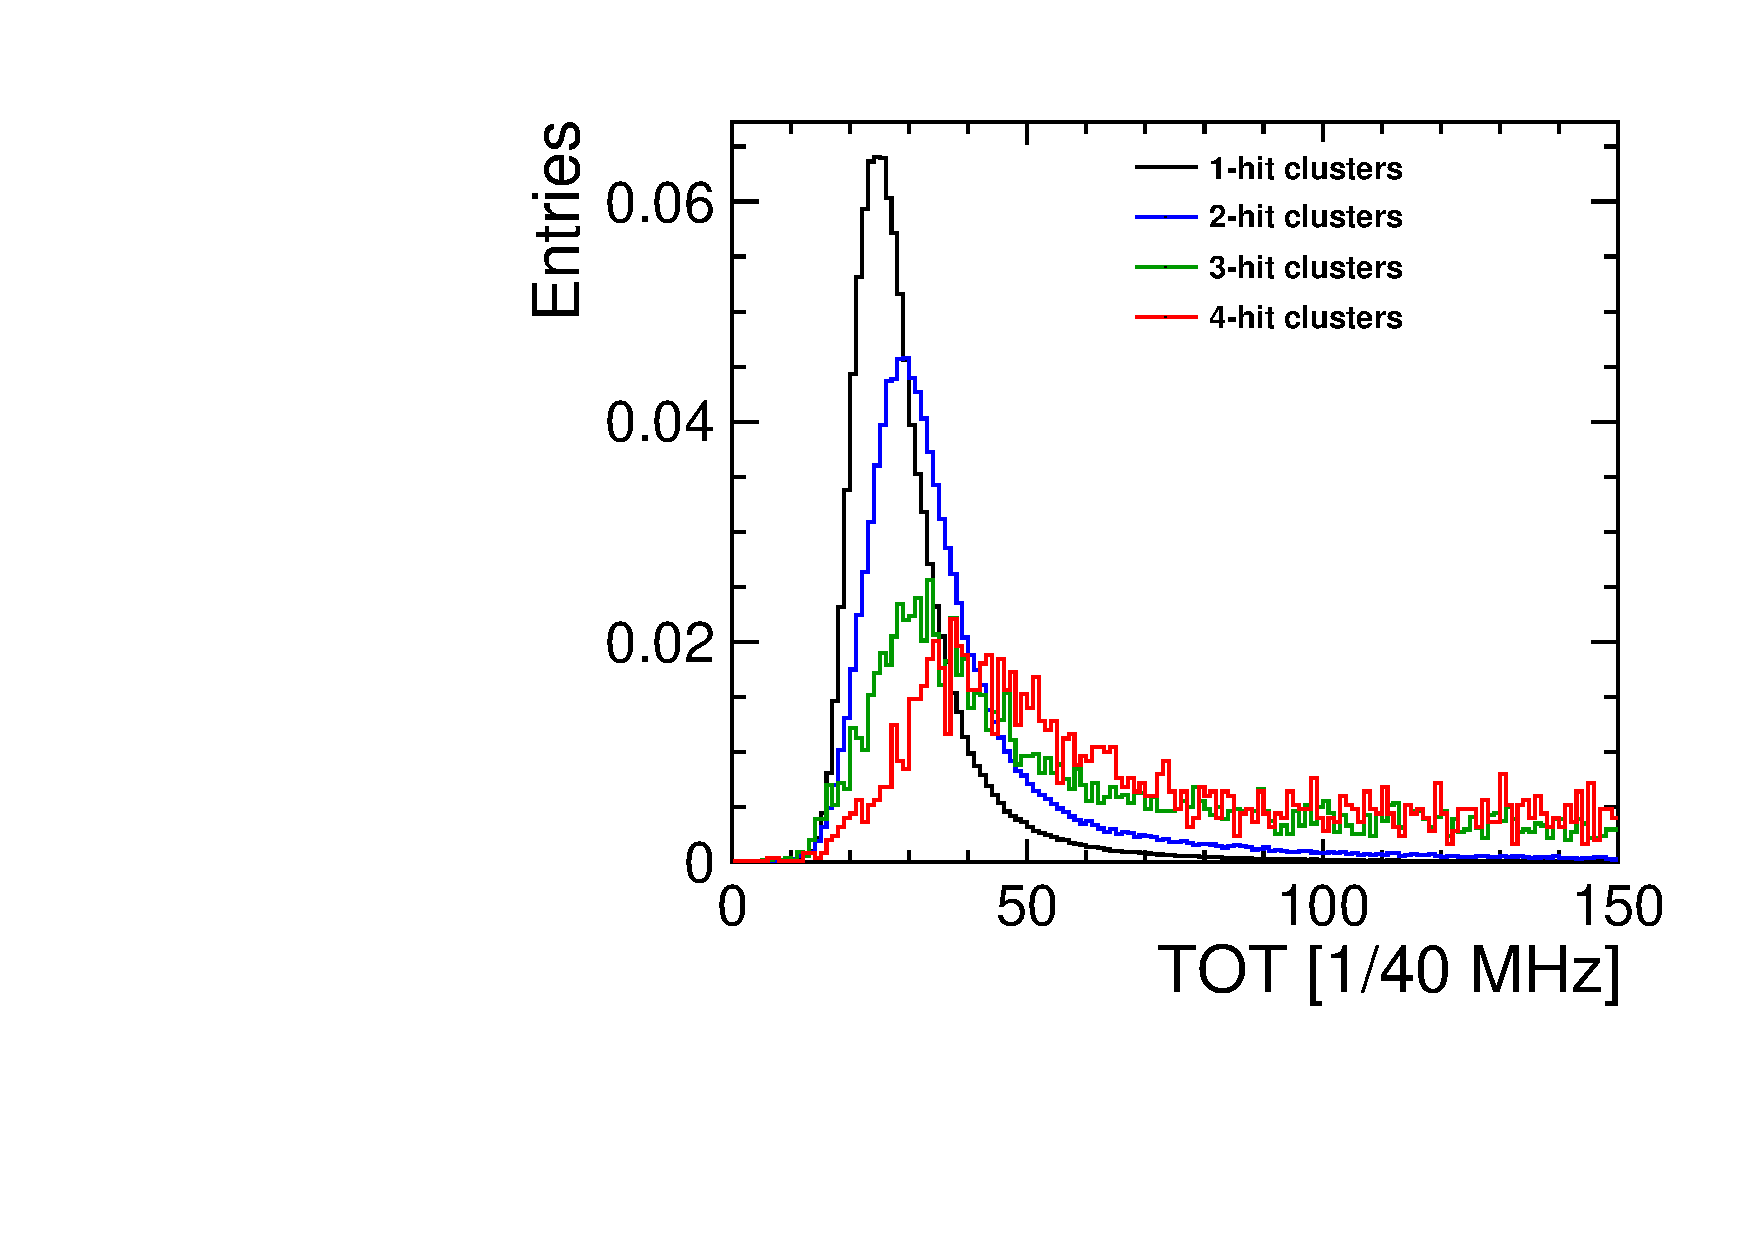
\includegraphics[width=\textwidth]{./figures/Calibration/TOT_Clusters_W0019_C07.pdf}
%     \caption{}
%   \end{subfigure}\hfill
%   \begin{subfigure}[b]{0.32\textwidth}
%     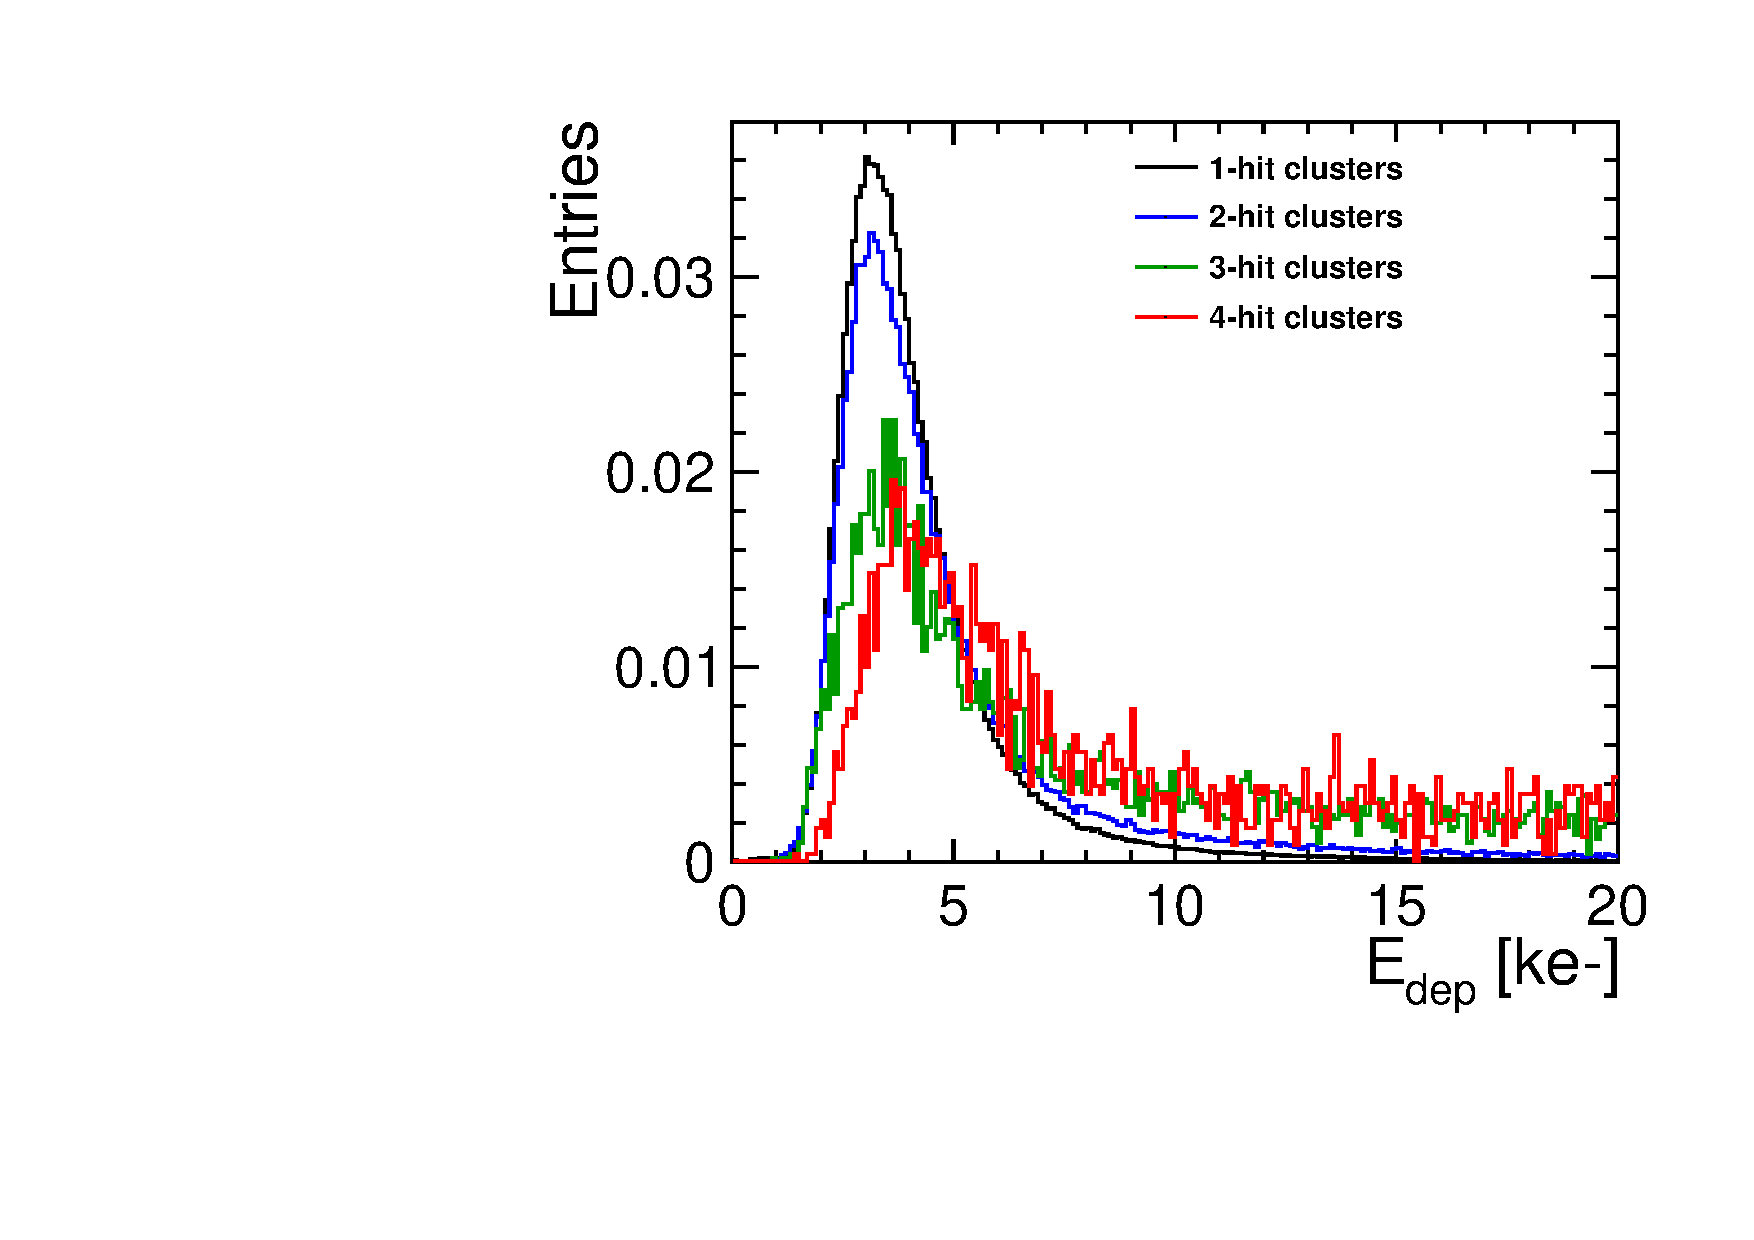
\includegraphics[width=\textwidth]{./figures/Calibration/Edep_Clusters_W0019_C07.pdf}
%     \caption{}
%   \end{subfigure}\hfill
%   \begin{subfigure}[b]{0.32\textwidth}
%     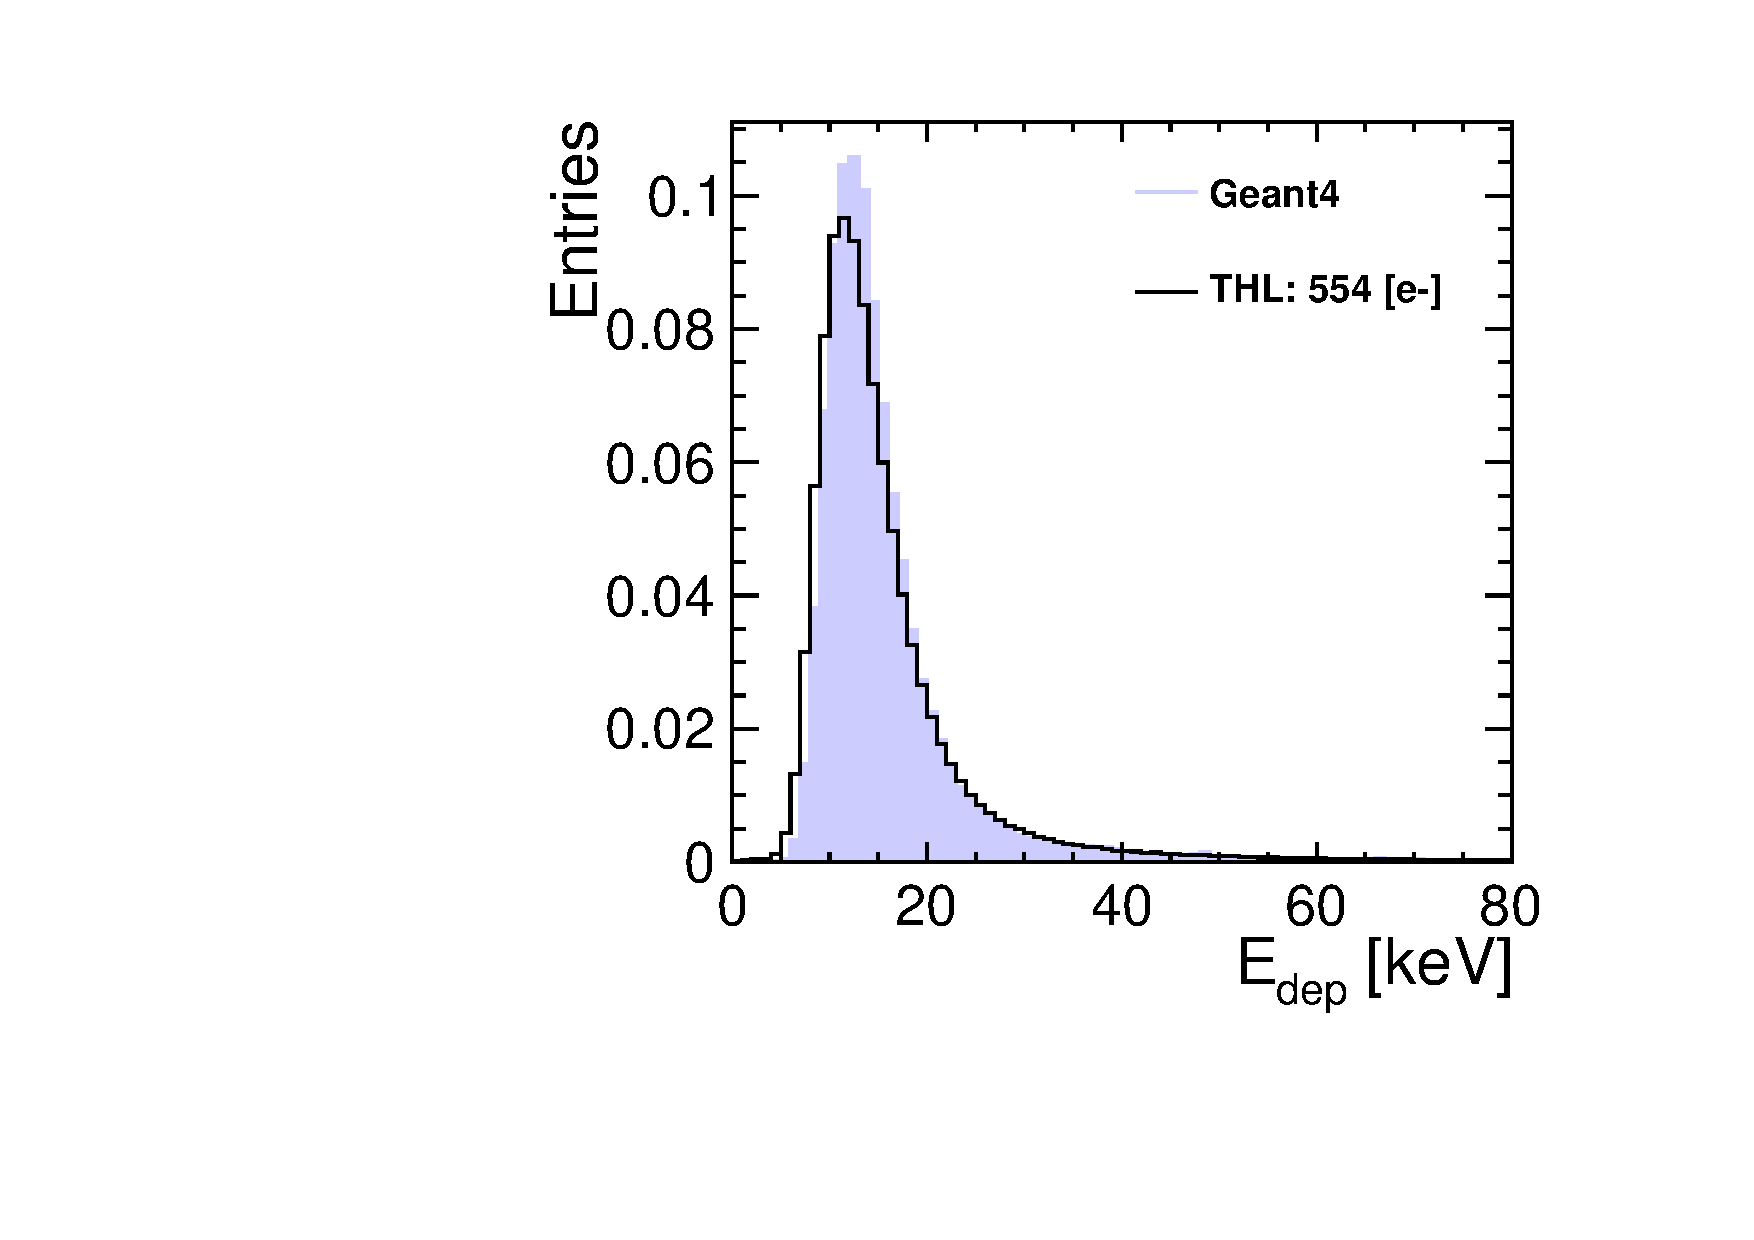
\includegraphics[width=\textwidth]{./figures/Calibration/Edep_G4_W0019_C07.pdf}
%     \caption{}
%   \end{subfigure}
%   \caption{Energy deposition and comparison to
%     \textsc{Geant4}. W0019\_C07, Run 902, THL=1148.}
%   \label{fig:EdepW19C7}
% \end{figure}


% \begin{figure}[htbp] \centering
%   \begin{subfigure}[b]{0.32\textwidth}
%     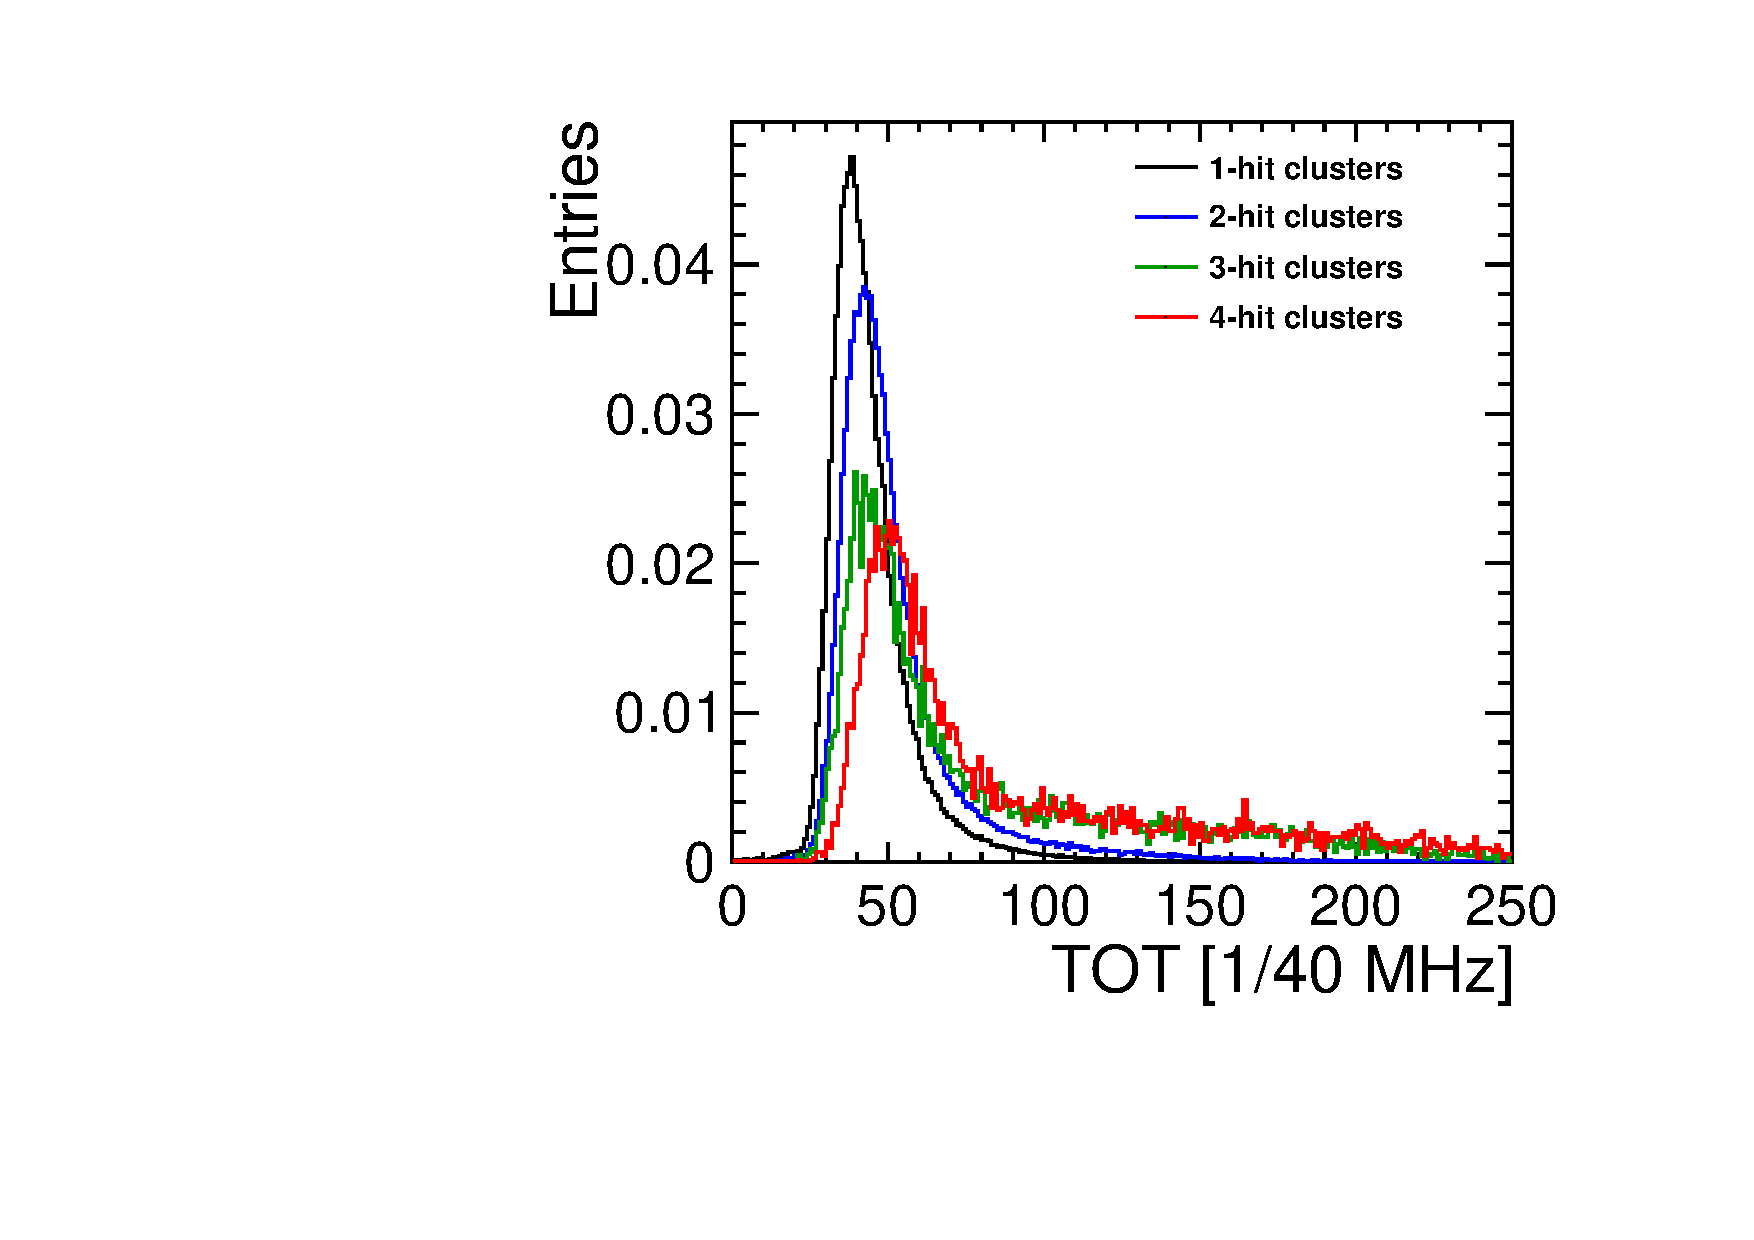
\includegraphics[width=\textwidth]{./figures/Calibration/TOT_Clusters_W0005_E02.pdf}
%     \caption{}
%   \end{subfigure}\hfill
%   \begin{subfigure}[b]{0.32\textwidth}
%     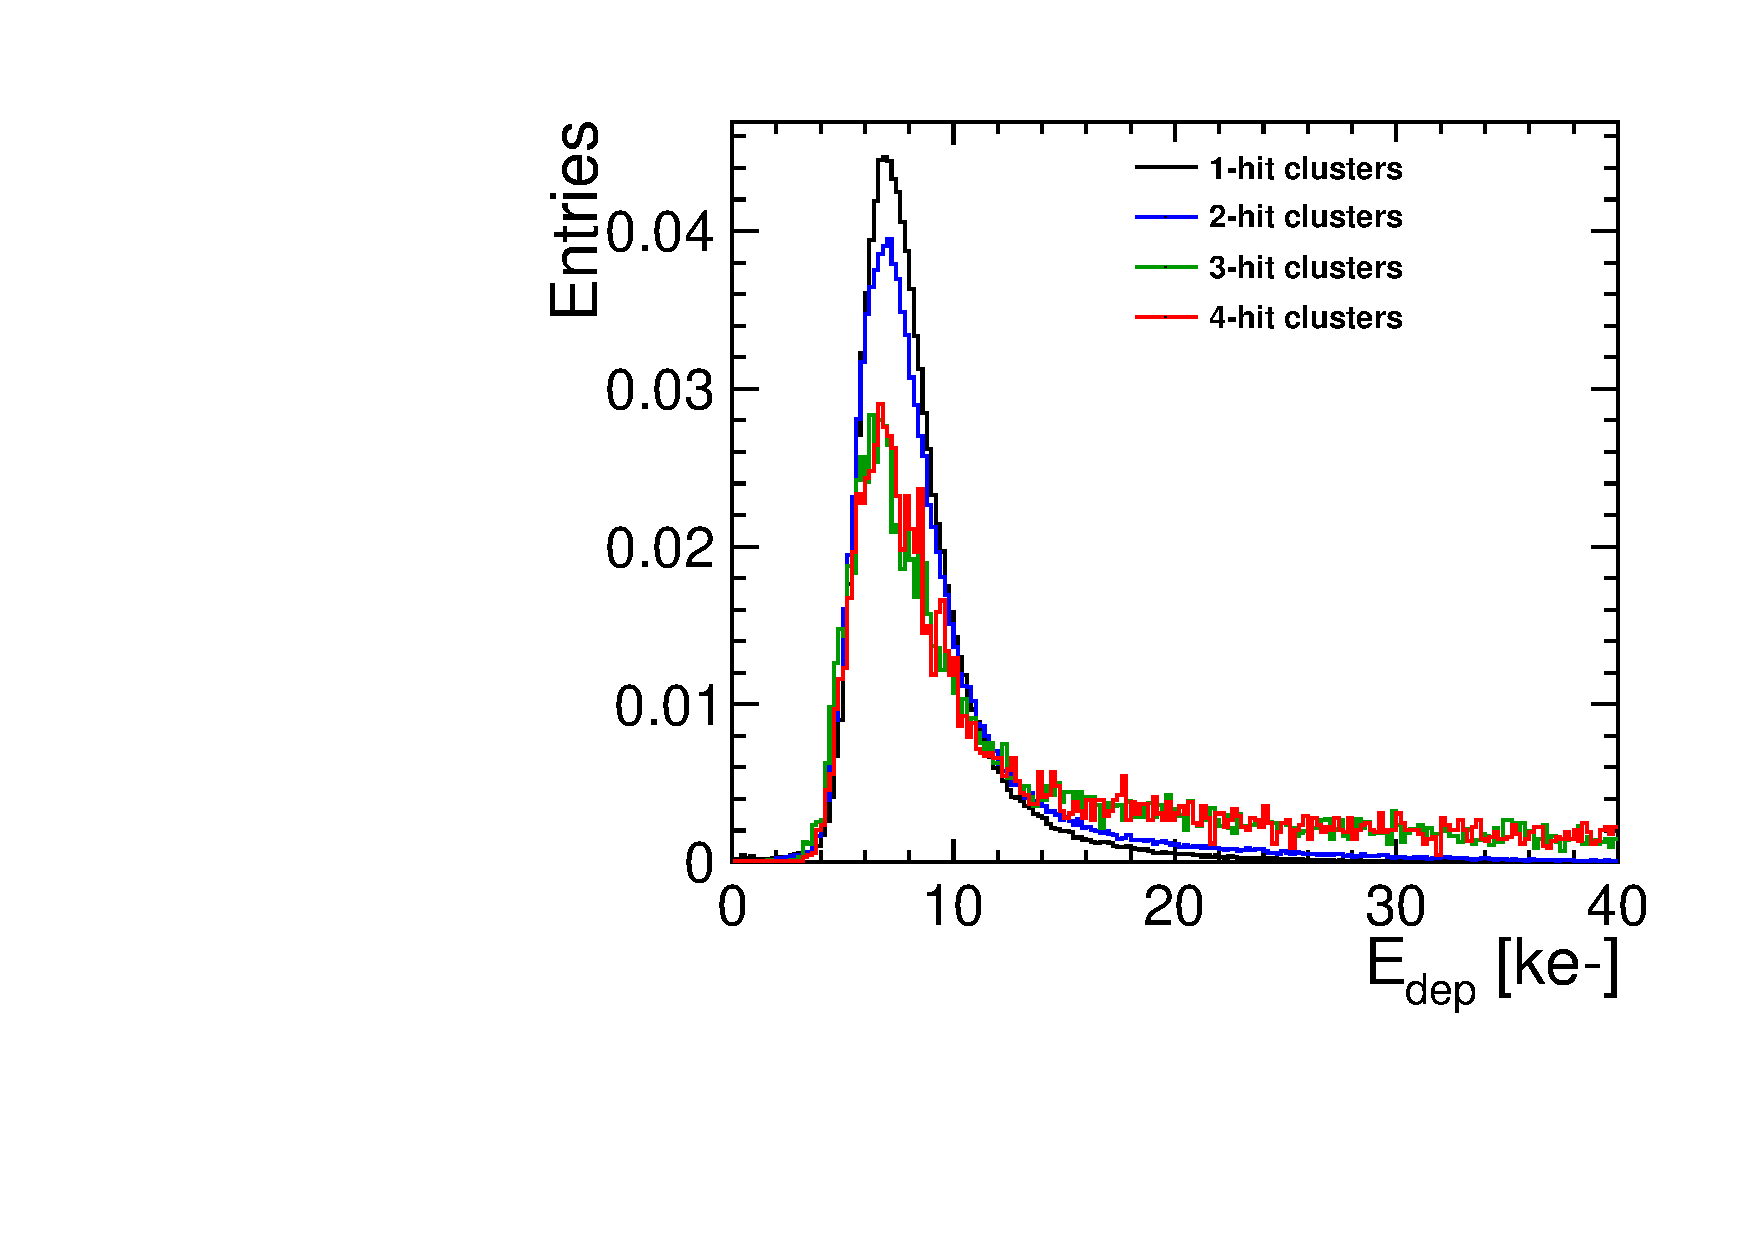
\includegraphics[width=\textwidth]{./figures/Calibration/Edep_Clusters_W0005_E02.pdf}
%     \caption{}
%   \end{subfigure}\hfill
%   \begin{subfigure}[b]{0.32\textwidth}
%     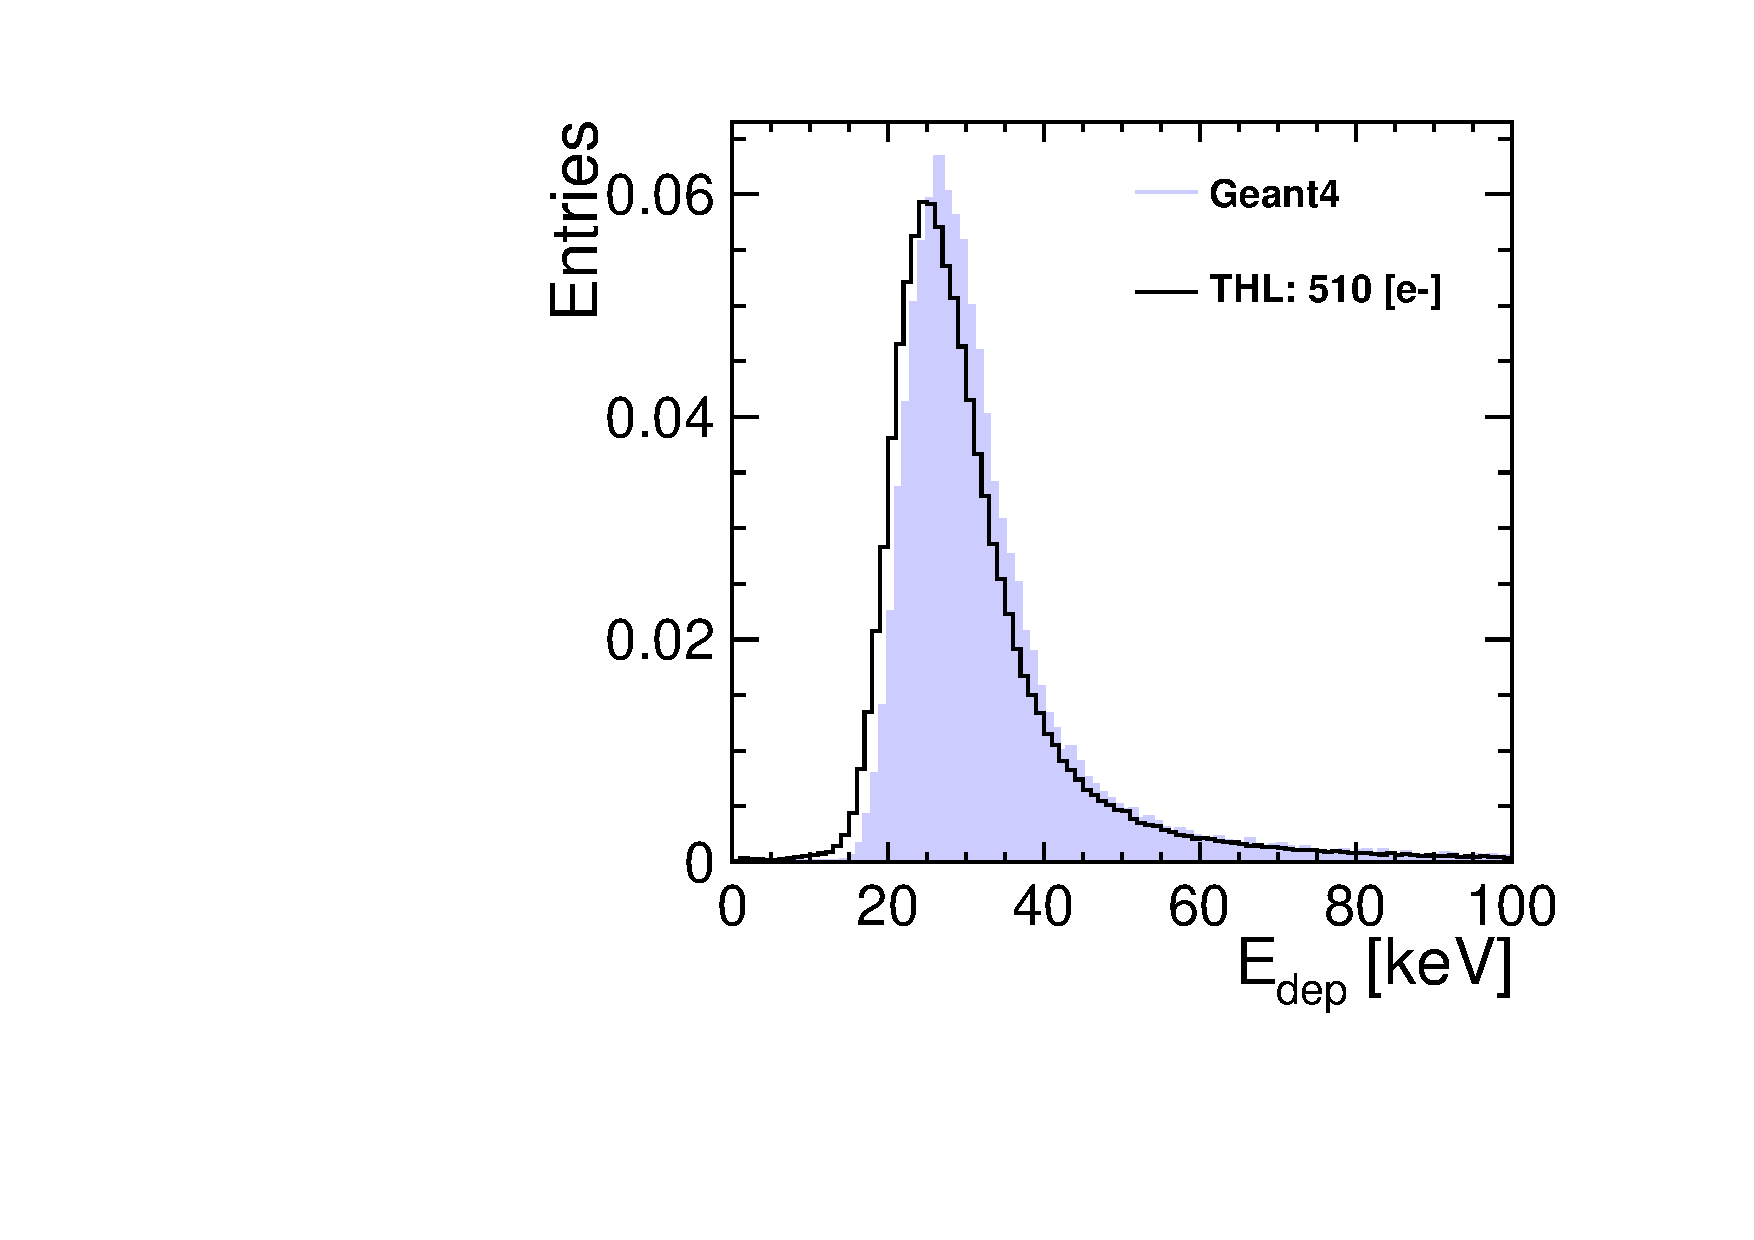
\includegraphics[width=\textwidth]{./figures/Calibration/Edep_G4_W0005_E02.pdf}
%     \caption{}
%   \end{subfigure}
%   \caption{Energy deposition and comparison to
%     \textsc{Geant4}. W0005\_E02, Run 661, THL=1160.}
%   \label{fig:EdepW5E2}
% \end{figure}

% \begin{figure}[htbp] \centering
%   \begin{subfigure}[b]{0.32\textwidth}
%     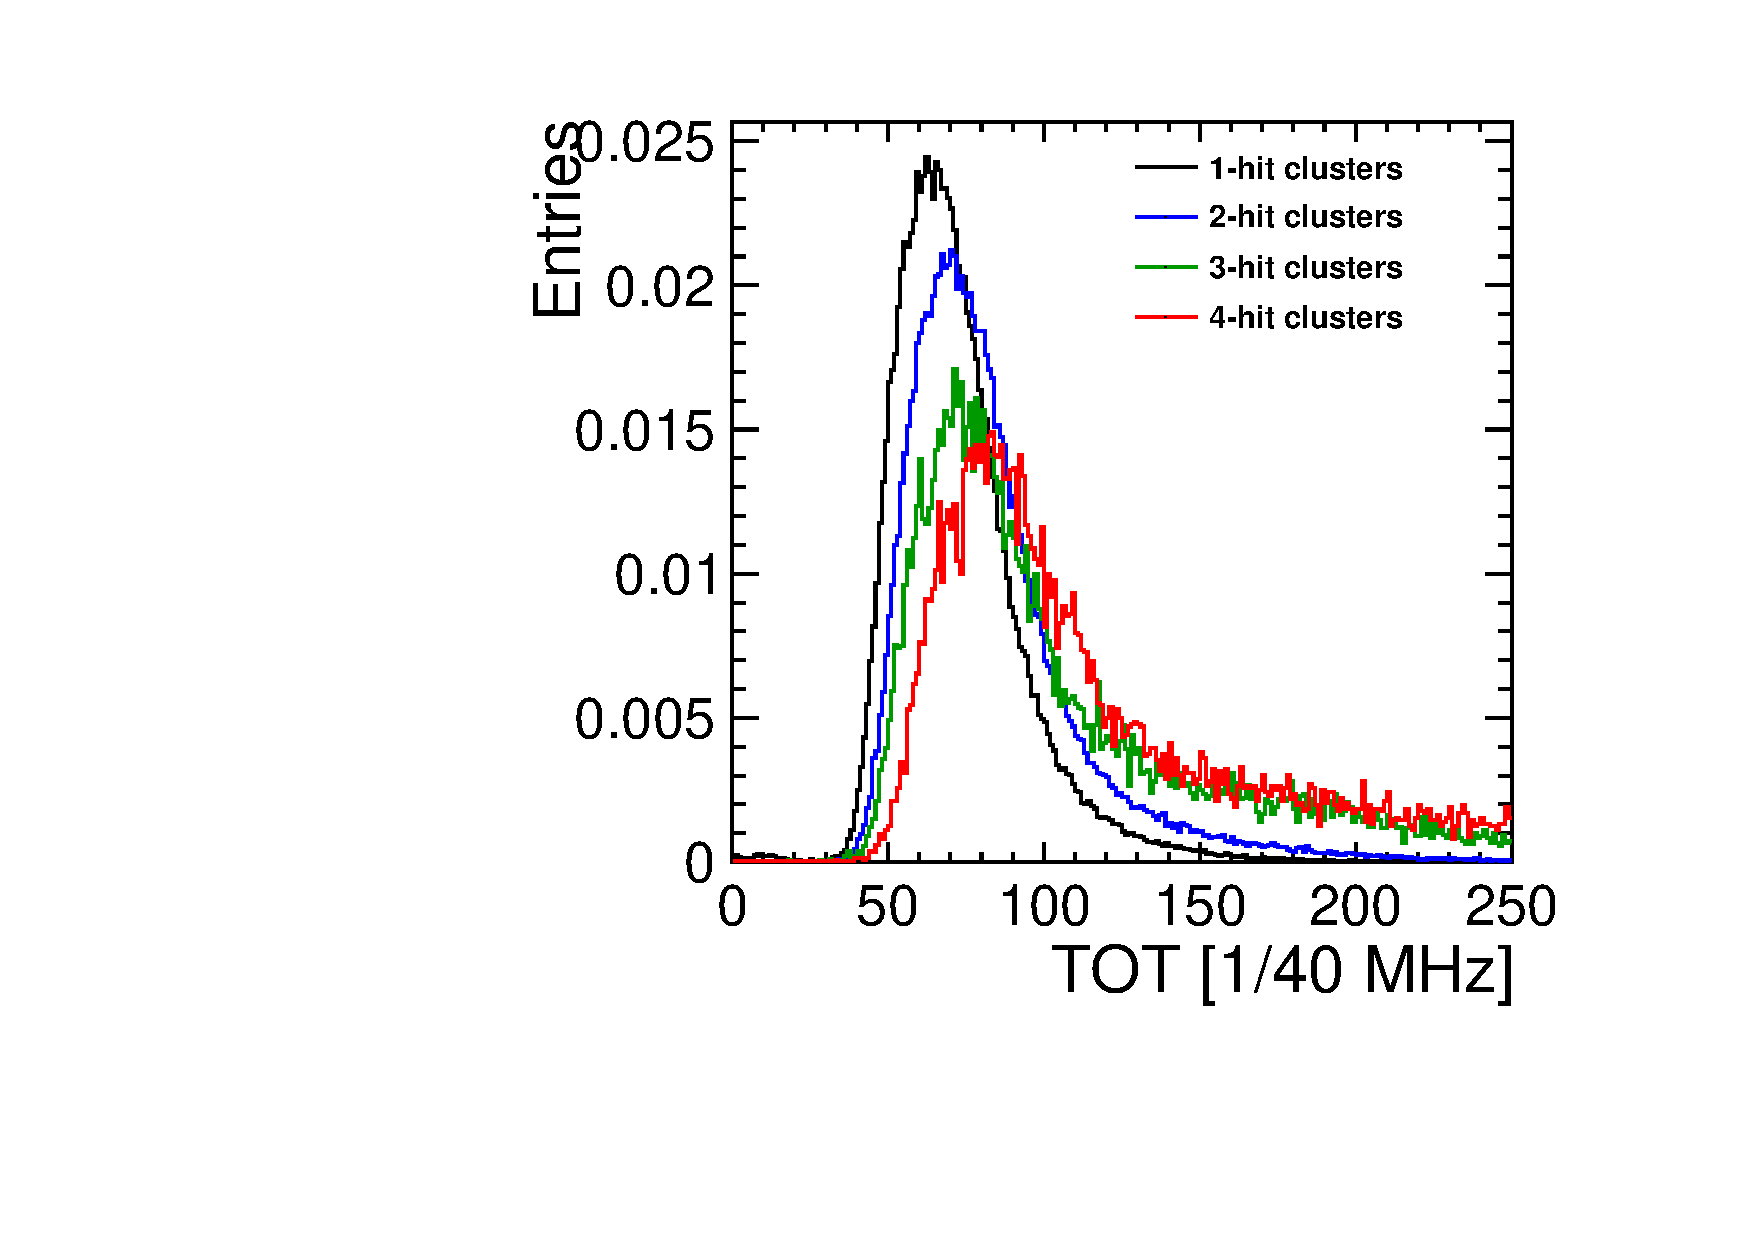
\includegraphics[width=\textwidth]{./figures/Calibration/TOT_Clusters_W0005_F01.pdf}
%     \caption{}
%   \end{subfigure}\hfill
%   \begin{subfigure}[b]{0.32\textwidth}
%     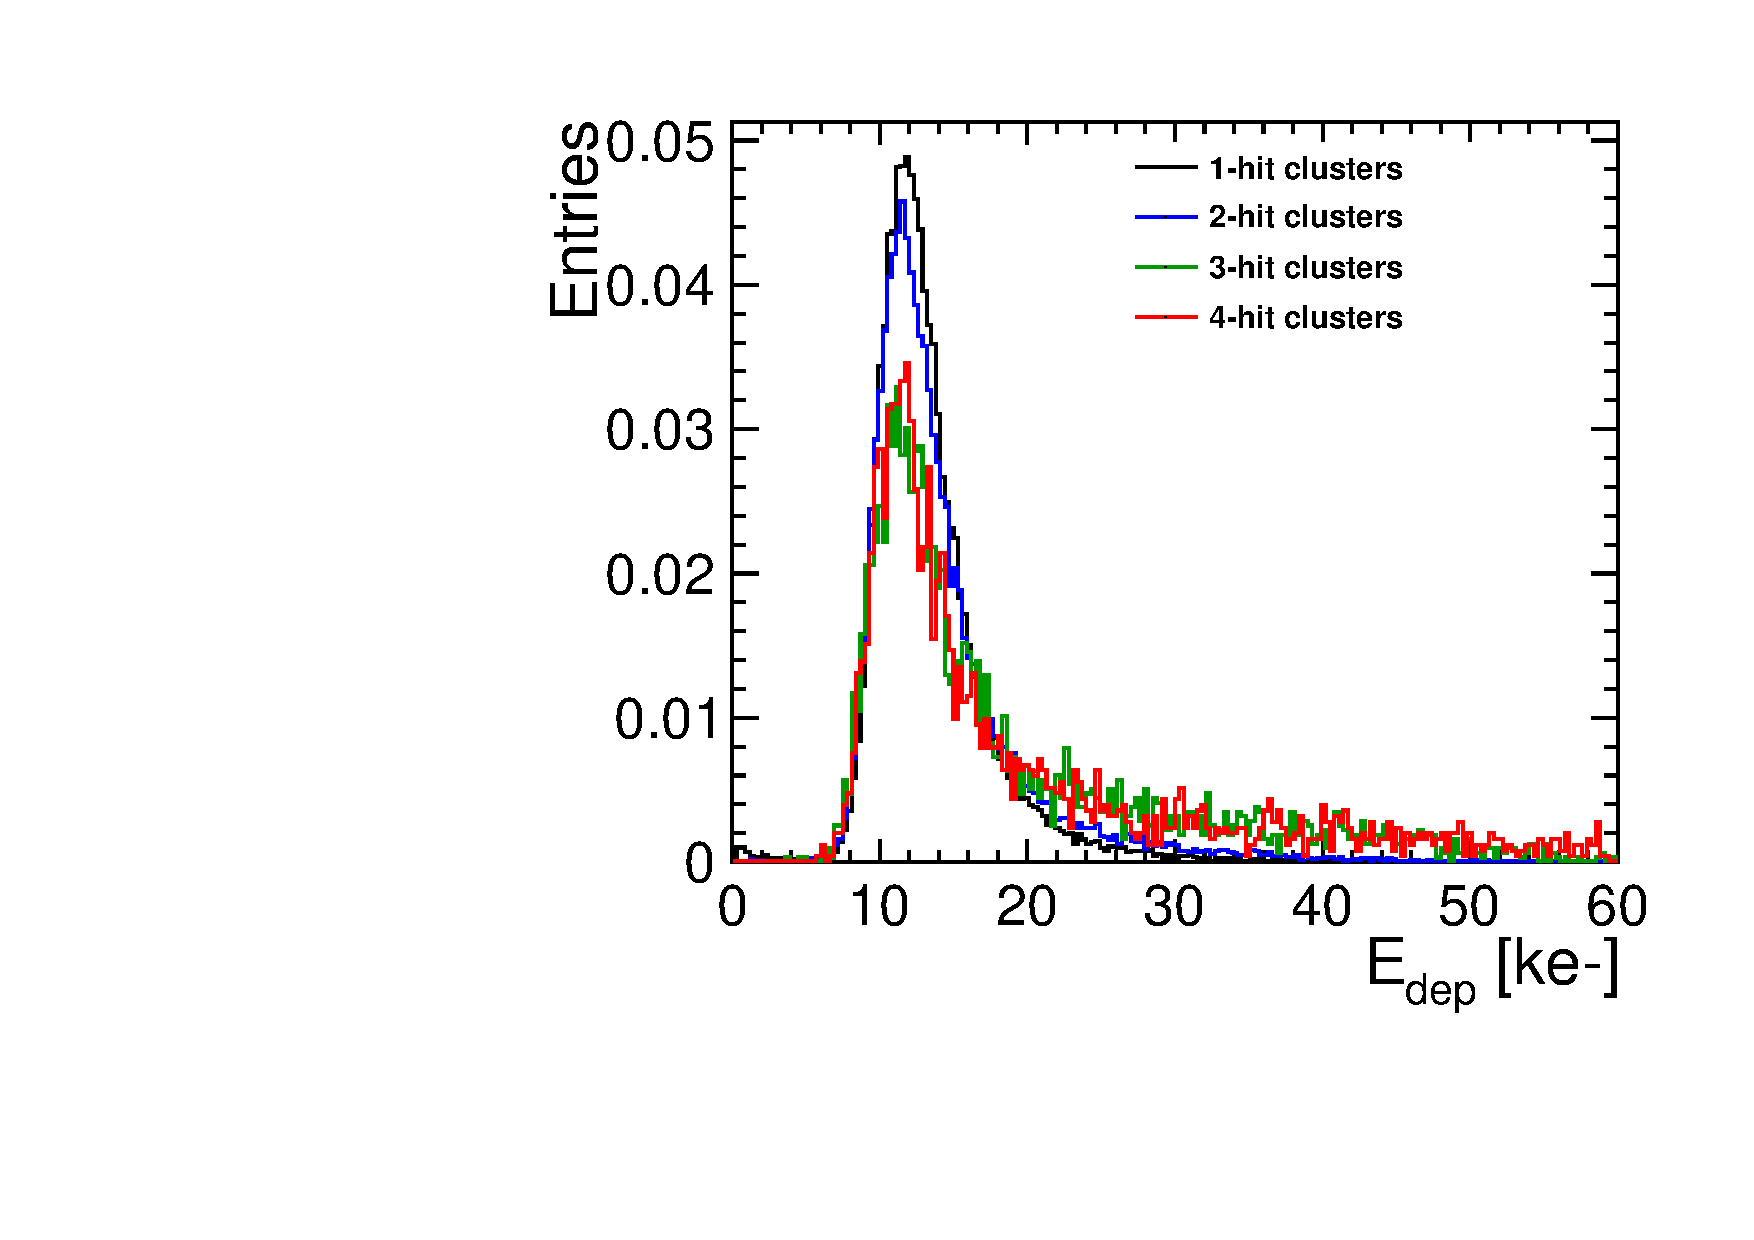
\includegraphics[width=\textwidth]{./figures/Calibration/Edep_Clusters_W0005_F01.pdf}
%     \caption{}
%   \end{subfigure}\hfill
%   \begin{subfigure}[b]{0.32\textwidth}
%     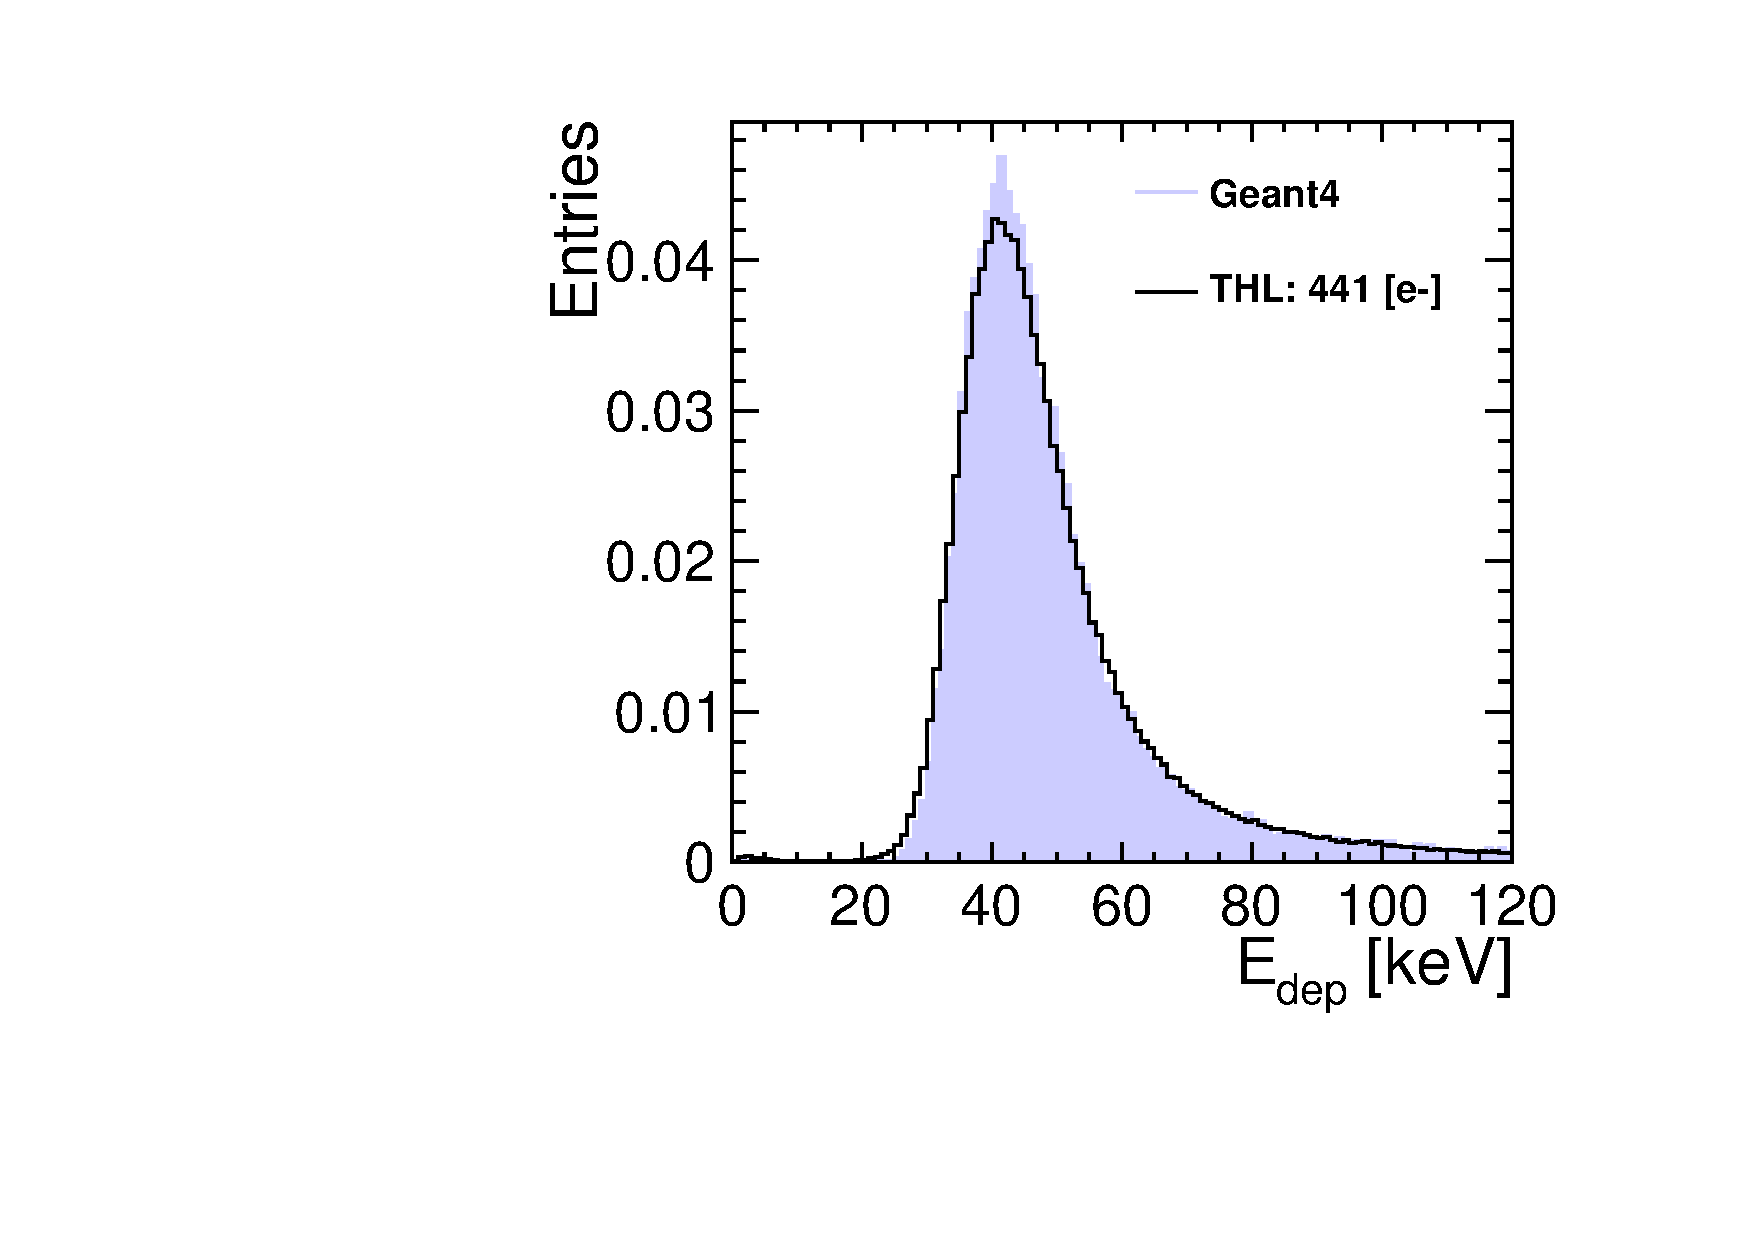
\includegraphics[width=\textwidth]{./figures/Calibration/Edep_G4_W0005_F01.pdf}
%     \caption{}
%   \end{subfigure}
%   \caption{Energy deposition and comparison to
%     \textsc{Geant4}. W0005\_F01, Run 761, THL=1153.}
%   \label{fig:EdepW5F1}
% \end{figure}
